% Do not change the options here
\documentclass[bsc,frontabs,parskip,deptreport]{infthesis}

\usepackage{graphicx}
\usepackage{subfig}
\usepackage[%  
    colorlinks=true,
    pdfborder={0 0 0},
    linkcolor=black,
    citecolor=blue
]{hyperref}
\usepackage{natbib}
\usepackage{csvsimple}
\usepackage{fancyvrb}
\citestyle{acmauthoryear}
% \setcitestyle{authoryear,comma,open={(},close={)}} 

\def\sectionautorefname{Section}	
\def\chapterautorefname{Chapter}
\def\subsectionautorefname{Section}
\def\subfigureautorefname{Figure}
\def\tableautorefname{Table}

\newcommand{\coderepo}{\href{https://github.com/LasseWolter/laughter-detection-icsi}{codebase}}

\newcommand{\confmatrixcaption}{Each row shows the percentage of laughter segments classified as a certain subclass for a given threshold (see \autoref{sec:conf-matrix}).}

\begin{document}
\begin{preliminary}
\title{A Machine Learning Model for Laughter Detection}

\author{Lasse Wolter}

% to choose your course
% please un-comment just one of the following
%\course{Artificial Intelligence}
\course{Artificial Intelligence and Computer Science}
%\course{Artificial Intelligence and Mathematics}
%\course{Artificial Intelligence and Software Engineering}
%\course{Artificial Intelligence with Management}
%\course{Cognitive Science}
%\course{Computer Science}
%\course{Computer Science and Management Science}
%\course{Computer Science and Mathematics}
%\course{Computer Science and Physics}
%\course{Computer Science with Management}
%\course{Software Engineering}
%\course{Software Engineering with Management}

\project{4th Year Project Report}

\date{\today}

\abstract{

% This skeleton demonstrates how to use the \texttt{infthesis} style for
% undergraduate dissertations in the School of Informatics. It also emphasises the
% page limit, and that you must not deviate from the required style.
% The file \texttt{skeleton.tex} generates this document and can be used as a
% starting point for your thesis. The abstract should summarise your report and
% fit in the space on the first page.
}

\maketitle

\section*{Acknowledgements}


\setcounter{tocdepth}{1} % Don't include subsections
\tableofcontents
\end{preliminary}


% The preliminary material of your report should contain:
% \begin{itemize}
% \item
% The title page.
% \item
% An abstract page.
% \item
% Optionally an acknowledgements page.
% \item
% The table of contents.
% \end{itemize}

\chapter{Introduction} \label{sec:intro}

The initial title of the project was \textit{A Zoom filter for applause and laughter}. The idea of this project was to create a third option for video-meeting participants. In addition to \texttt{mute} and \texttt{unmute}, a new option called \texttt{filtered} should be added.
In \texttt{filtered}-mode, a user is automatically unmuted when laughter or applause is detected. 
The motivation behind this feature is a more engaging speaker experience in virtual conferences. The project's supervisor is regularly involved in such conferences and wishes that reactions like laughter and applause were audible to him.

To achieve the original goal, a real-time machine learning model detecting laughter and applause is required.  
This project narrows the scope to a machine learning model for laughter detection. Real-time constraints are considered theoretically (\autoref{sec:real-time}) but adapting the model implementation for real-time usage is left for future work.
The project was renamed to \textit{A machine learning model for laughter detection} as the focus of the project was set on laughter detection; the beginning of the thesis briefly covers some aspects of applause detection. 

Due to poor results of the final model, this thesis outlines the process I have taken, issues I faced and states my final hypothesis about the results: 

\textit{``A significant number of non-transcribed regions in the ICSI corpus are not actually silence; they are quieter recordings of speech by other participants. Thus, the assumption that non-transcribed regions and laughter can be easily distinguished is wrong."}

The main achievements of this project are:
\begin{enumerate}
  \item Evaluation of an existing laughter detection model on the whole ICSI meeting corpus (\autoref{cha:model-evaluation})
  \item Creation of a machine learning pipeline for training and evaluating laughter recognition on the ICSI meeting corpus (\autoref{cha:retraining})
  \begin{itemize}
      \item This code is publicly available for future work (\coderepo)
  \end{itemize}
  \item Investigation of model performance with varying training data (\autoref{cha:experiments})
  \begin{itemize}
      \item Includes the process of coming up with my final hypothesis 
  \end{itemize}
\end{enumerate}


The thesis starts off with a review of existing approaches about laughter and applause detection (\autoref{cha:bg}). It introduces some evaluation metrics used and gives a more detailed view of the model introduced by \citet{gillick2021robust} which is the foundation for my work. \autoref{cha:model-evaluation} takes the best model from \citet{gillick2021robust}, trained on the Switchboard corpus \citep{switchboard-corpus}, and evaluates it on the ICSI corpus \citep{morgan2001meeting}. The evaluation was revised throughout the project. \autoref{cha:model-evaluation} includes a comparison of these revisions and an analysis of the overall poor performance of the model, which was made at the time of evaluation and does not include my final insights about the corpus.

Due to the poor performance described in \autoref{cha:model-evaluation}, I retrained the model on the ICSI corpus. \autoref{cha:retraining} outlines how I first failed to use the existing training code from \citet{gillick2021robust} and then adapted it using \texttt{Lhotse} \citep{zelasko2021lhotse}, a new audio processing library, which I ended up contributing to \autoref{app:lhotse-contrib}.

\autoref{cha:experiments} presents experiments investigating the impact of training data on the model output. It also compares the newly trained models with the original model evaluated in \autoref{cha:model-evaluation}. We find that models retrained on the ICSI corpus perform significantly better than the pre-trained model by \citet{gillick2021robust}, trained on the Switchboard corpus. Nevertheless, the model performance remains unusable for integration in a video call system. Therefore, \autoref{sec:silence-regions} includes some manual investigation of the corpus data. In hindsight, these experiments should have been conducted earlier. 

Lastly, \autoref{cha:practicality} investigates the practicality of the \texttt{filtered} option using laughter detection within a video call system; this includes real-time and privacy considerations as well as alternative solutions. The chapter concludes with suggestions for future work and a latency estimate of the model used in this thesis for future reference. 

Throughout the report I regularly mention discussions. These refer to the biweekly meetings with my first and second supervisor, where I presented my progress. For each meeting I prepared a set of slides which are available at \href{https://github.com/LasseWolter/honours-project-21-22/tree/main/Meeting_Notes}{this public github repository}.
The final laughter recognition codebase is published \href{https://github.com/LasseWolter/laughter-detection-icsi}{here}.


\chapter{Applause and Laughter Detection} \label{cha:bg}
Automatic applause and laughter detection isn't a new idea. Nevertheless, the research in these two areas is usually done separately; there are a few papers that cover both. One of the most popular papers is \citet{cai2003highlight} who used sound effect detection - which included laughter and applause - for video summarisation and highlight extraction.
Apart from this and a few other papers, most research only covers one of the two domains, either applause or laughter. Thus, the review covers them in separate sections. A third section for evaluation metrics was added to introduce some of the core metrics used in this field. 

\section{Laughter Detection} \label{sec:bg-laughter}
The investigation of laughter's acoustic features reaches back three decades \citep{bickley1992acoustic}.
In the early 2000s, the first attempts of laughter detection in conversational speech classified presegmented audio data \citep{kennedy2004laughter, truong2005automatic}. These models could only state whether laughter occurred within a given segment. The determination of segment boundaries of laughter events was not considered. 
Corpora used in these papers include the development data from the 2004 Spring NIST Rich Transcription Evaluation \citep{nist-recordings}, the Dutch CGN corpus \citep{oostdijk2000spoken} as well as the ICSI Meeting Recorder corpus \citep{morgan2001meeting}. 

Two examples of such classification of presegmented audio data are \citet{kennedy2004laughter} and \citet{truong2005automatic}. 
Even though both of these models classified presegmented audio there were some significant differences. 
Firstly, the definition of laughter and the motivation behind the research differed.
While \citet{kennedy2004laughter} define laughter events as `points in the meeting where more than one person laughs', \citet{truong2005automatic} considered one person laughing as a laughter event.
\citet{kennedy2004laughter} did not specify a particular motivation whereas \citet{truong2005automatic} stated the long-term goal of investigating `paralinguistic events' - laughter being one of them - to classify the speaker's emotional state.   

Secondly, there was a difference between the best performing features and predictors.  
Features tried include Mel Frequency Cepstral Coefficients (MFCCs), delta MFCCs (MFCC derivatives), spatial cues, modulation spectrum features and Perceptual Linear Prediction(PLP) features. 
\citet{kennedy2004laughter} got the best results using MFCCs as features and a Support Vector Machine (SVM) for decision making.
In contrast, \citet{truong2005automatic} used Perceptual Linear Prediction (PLP) features with Gaussian Mixture Models (GMM) for classification. 

\citet{truong2007automatic} continued their research and stated that spectral features alone (such as PLP and MFCCs) can be used to discriminate between laughter and speech but a significant improvement can be achieved when using prosodic features - features relating to rhythm and intonation.

In 2006, \citet{knox2006automatic} was the first to do laughter recognition without the need for presegmented audio data.  
Their goal was to obtain accurate interval boundaries of laughter segments.
One limiting factor for the precision of these boundaries is the frame size. 
When \citet{knox2006automatic} first experimented with SVMs similar to \citet{kennedy2004laughter}, they realised that the time to compute the features and train the SVM increased significantly with decreasing frame size. 
This is because aggregate statistics need to be calculated and stored for each frame of training data.  
On the contrary, a neural network trained with features from a context window can directly use the features of each frame without aggregating them.  

To obtain frame-level training labels for the ICSI dataset, \citet{knox2006automatic} first removed all segments that contained both speech and laughter within one transcription segment, because the segment boundaries of such laughter occurrences could not be identified. 
The remaining audio data could be accurately separated into laughter and non-laughter segments based on the ICSI transcriptions. Each of these segments was divided into non-overlapping 10ms frames and labeled accordingly.

The model was trained to classify each 10ms frame using a window of 75 frames around the target frame - 37 before and 37 after the frame (\autoref{fig:knox_window}).
This way an accurate prediction of laughter boundaries of up to 10ms was possible. 
The features investigated by Knox and Mirghafori are MFCCs, AC PEAK, F0 and RMS as well as their corresponding delta and delta-delta features (first and second derivatives of the features).
They first trained four separate neural networks each one taking one of the mentioned features as input.
Afterwards, they combined the different models by using their output as input for another, smaller neural network.
The best results were obtained by combining the outputs of three NN-systems which used delta MFCCs, AC PEAK and F0 as features, respectively.
By training and evaluating separate neural networks for each type of feature first, Knox and Mirghafori observed that MFCCs have the most discriminative power which aligns with prior research by \citet{kennedy2004laughter}.

\begin{figure}[htp]
    \centering
    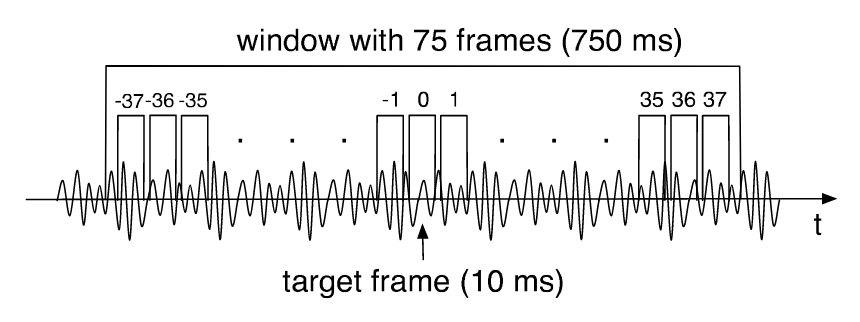
\includegraphics[width=10cm]{imgs/Knox_window.png}
    \caption{Frame window used by \citet{knox2006automatic}}
    \label{fig:knox_window}
\end{figure}

A survey from \citet{cosentino2016quantitative} investigates research on laughter and laughter detection in different fields up to that time.
This survey covers different detection methods using visual, acoustic and sensory data.
\citet{cosentino2016quantitative} found that using solely acoustic features best performance is obtained by using MFCCs and PLPs as features and combining the resulting classifier with ones that also use prosodic features.
This aligns with findings from prior research \citep{truong2007automatic, knox2006automatic}.

More recent research by \citet{gillick2021robust} finds that features learned from spectrograms using deep convolutional networks outperform previous approaches based on MFCCs. 
They hypothesised that models using MFCCs are more prone to pick up surface level characteristics of sound and thus, will be more sensitive to variations like background noise.
\citet{gillick2021robust} expected that features learned directly from the spectrogram are more representative of the actual laughter and thus, more robust to different environments. 
To test this hypothesis they trained three different models: a baseline feed-forward neural network with MFCC features from their existing research \citep{ryokai2018capturing}, a ResNet-18 \citep{he2016deep} model working directly on spectrogram data and the same ResNet model using augmented features. Augmentations applied include pitch-shifting, time-stretching, reverberation and SpecAugment \citep{park2019specaugment}. SpecAugment is a simple method to augment spectrograms by time warping, frequency masking and time masking. \autoref{fig:spec-augment} shows that frequency and time masking is done by blocking out certain spectrogram regions, vertically or horizontally. 

\begin{figure}[h!]
    \centering
    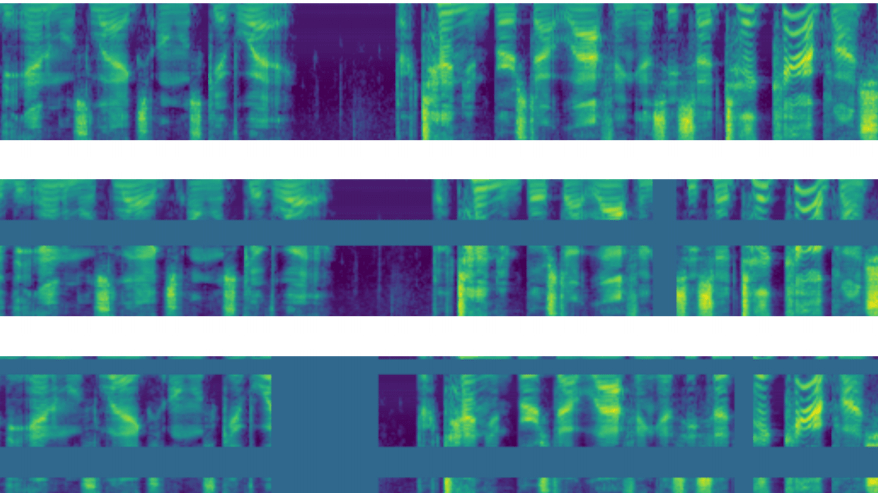
\includegraphics[width=13cm]{imgs/examples/spec_augment_example.png}
    \caption{SpecAugment example}
    \label{fig:spec-augment}
\end{figure}

\citet{gillick2021robust} trained their model on two corpora: the Switchboard corpus \citep{switchboard-corpus} and AudioSet \citep{googleaudioset}. They used Binary Cross Entropy loss for optimisation, which is explained in \autoref{sec:cross-entropy-loss}.
In contrast to prior work, they also evaluated the models on the corpus that it was not trained on.
This mismatch between training and testing data tries to resemble the difference between clean audio and real-world test data.

Their results (\autoref{fig:gillick-results}) mention strongly and weakly labeled data.
Weakly labeled means that only the presence or absence of an event is given, whereas strongly labeled data states precise boundaries.
AudioSet \citep{googleaudioset} is a weakly labeled corpus consisting of ten second segments sampled from YouTube videos. Each segment has one or more annotations like \texttt{laughter} or \texttt{wind}, which state that these sounds are present in the given segment. Since segments are sampled from a range of YouTube videos, domains in this corpus vary greatly.
The Switchboard dataset is a strongly labeled corpus consisting of telephone conversations between two individuals. Compared to AudioSet, the domain is homogeneous across all recordings and a transcription file provides precise boundaries for audio events.

\autoref{fig:gillick-results} shows that in all evaluations the baseline model using MFCC features and a feed-forward neural network is outperformed by the ResNet architecture in every metric, except the recall for the model trained on AudioSet and evaluated on the Switchboard test data. 
\citet{gillick2021robust} conclude that their ResNet-based model provides a robust, state-of-the-art laughter-detection algorithm that mitigates some of the problems of noisy real-world environments. This is one of the reasons why it is used as a basis for this project.

\begin{figure}[h!]
    \centering
    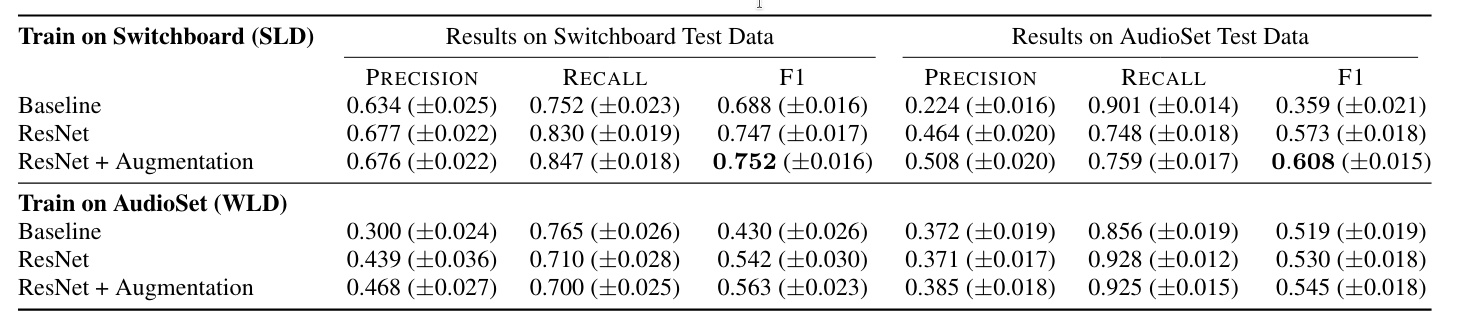
\includegraphics[width=14cm]{imgs/results/gillick_et_al.png}
    \caption{Results by \citet{gillick2021robust} with 95\% confidence intervals. Precision, Recall, and F1 scores are calculated as segment-based metrics (\autoref{sec:acc-prec-rec}). SLD=Strongly labeled data, WLD=weakly labeled data.}
    \label{fig:gillick-results}
\end{figure}

\section{Applause}
The following review is less exhaustive because this thesis focuses on laughter detection. Applause detection is a possible extension of the project to meet the original goal mentioned in \autoref{sec:intro}. 
More information on this decision can be found (\autoref{sec:model-and-data}).

As mentioned at the beginning of this chapter, in 2003 \citet{cai2003highlight} worked on the detection of sound events, including applause.
They used perceptual features and MFFCs as features, Hidden Markov Models (HMM) and Gaussian Mixture models (GMM) to model sound and log likelihood for decision making.
\citet{cai2003highlight} evaluated their system on a testing set consisting of 2 hours of video material from different programs.
For applause specifically, they achieved a precision of 87.37\% and a recall of 92.00\%.

In contrast, \citet{uhle2011applause} used MFCCs and low-level descriptors (LLD) to represent sound and passed these features to an Multi-Layer-Perceptron (MLP) or an SVM for classification.
The difference between the MLP and SVM classifier was rather small.
Uhle worked with a relatively small dataset consisting of 210 segments of 9-30s length. This equates to a total length between 31.5 min and 105 min.
On a rather small test (10\% of this dataset) Uhle achieved an accuracy of 95\% with a precision of 96.51\% and recall of 97.65\%.

A less complex approach for applause detection was presented by \citet{li2009characteristics}.
They used a manually created 4-layer decision tree to classify a given sound input as applause or not-applause.
Testing their model on 50 hours of meeting speech containing 500 applause segments ranging from 0.8s to 36s they were able to retrieve 491 of the 500 applause segments while incorrectly retrieving 38 non-applause segments.
This equates to a recall of 98.2\% and precision of 92.82\%. Li et al. also compared their less complex model to the HMM model proposed by \citet{cai2003highlight} and outperformed it while using less computational time.

\citet {manoj2011novel} proposed another approach based on manually created decision trees. They also compared it to a more complex model similar to the one proposed by \citet{cai2003highlight} - with the difference that this model only used GMMs, no HMMs.
Even though the decision tree stages were different to \citet{li2009characteristics} the findings are similar. The decision tree outperforms the more complex method using MFCCs and GMMs.  

\section{Evaluation Metrics} \label{theory}
\subsection{Accuracy, Precision and Recall} \label{sec:acc-prec-rec}
Accuracy, precision and recall are standard metrics for performance evaluation.
All three metrics are calculated by comparing the predicted class labels to the true class labels.
This section states the formulae, their meaning for our use case and the advantages of one metric over the other.
Let:
\begin{enumerate}
    \item $TP$: True Positives - laughter samples correctly classified as laughter,
    \item $FP$: False Positives - non-laughter samples incorrectly classified as laughter,
    \item $TN$: True Negatives - non-laughter samples correctly classified as non-laughter,
    \item $FN$: False Negatives - laughter samples incorrectly classified as non-laughter.
\end{enumerate}
\textbf{Accuracy}: Percentage of correctly classified samples (laughter and non-laughter) over the total number of samples.
$$Accuracy = \frac{TP+TN}{TP+TN+FP+FN}$$
\textbf{Precision}: Percentage of correctly classified laughter samples over all samples predicted as laughter.
$$Precision = \frac{TP}{TP+FP}$$
\textbf{Recall}: Percentage of correctly classified laughter samples over all laughter-samples.
$$Recall = \frac{TP}{TP+FN}$$

For our use case, we are interested in continuous audio data, but all metrics presented above are calculated on discrete data points. We make use of segment-based metrics suggested by \citet{mesaros2016metrics} which splits a continuous audio stream into fixed-sized segments (e.g. 10ms). These fixed-sized segments are treated as separate instances and build the base-unit for our evaluation (e.g. 1s laughter will become 100 units of laughter). Assuming that 0.6s of are predicted correctly this would yield 60 $TP$ and 40 $FP$.
\citet{gillick2021robust} used the same approach for their evaluations.

Accuracy is a good metric if classes are balanced. In our use case, the two classes are highly imbalanced; laughter only occurs a few times in a long audio stream. If we choose a very high threshold the model predicts all segments as non-laughter. This leads to a large number of true negatives which skews the accuracy. This model with no skill gets high accuracy.
Considering the same example, the precision will be 100\% as well, but the recall will be 0\% because the model did not retrieve any laughter segments correctly. 
The other extreme is given by a threshold of 1. The model will predict everything as laughter, which leads to a low accuracy and low precision because only the few seconds of laughter in the whole meeting are classified correctly. The recall will be 100\% because the model retrieved all laughter that occurs. 
To capture the range between these two extremes a precision-recall curve is a useful tool. Precision recall curves plot the precision against the recall for a range of thresholds (e.g. \autoref{fig:prec-recall-example}). This provides a more detailed view of the model performance and answers questions like: "What is the precision of the model if we require a minimum recall of 80\%".

\begin{figure}[h!]
    \centering
    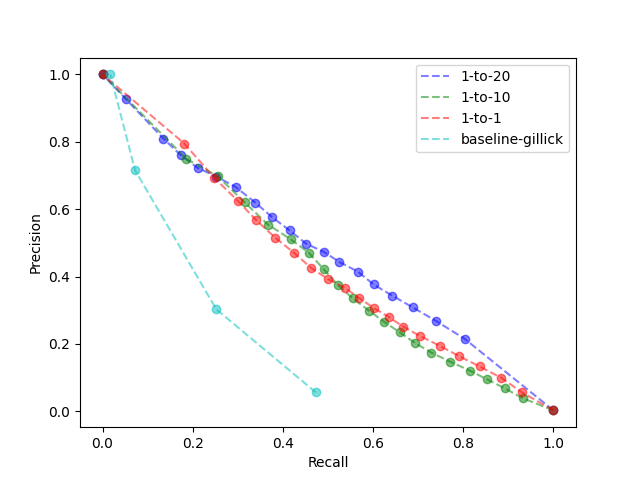
\includegraphics[width = 10cm]{imgs/prec-recall/exp1-random/dev_compare_class_balance_dev_set.png}
    \caption{Example precision-recall curve showing precision and recall of different models. Taken from \autoref{cha:experiments}.}
    \label{fig:prec-recall-example}
\end{figure}

To conclude, for our use case reporting precision and recall across a range of thresholds is a more expressive metric than accuracy.

\subsection{Confusion Matrix} \label{sec:conf-matrix}
\begin{figure}[h!]
    \centering
    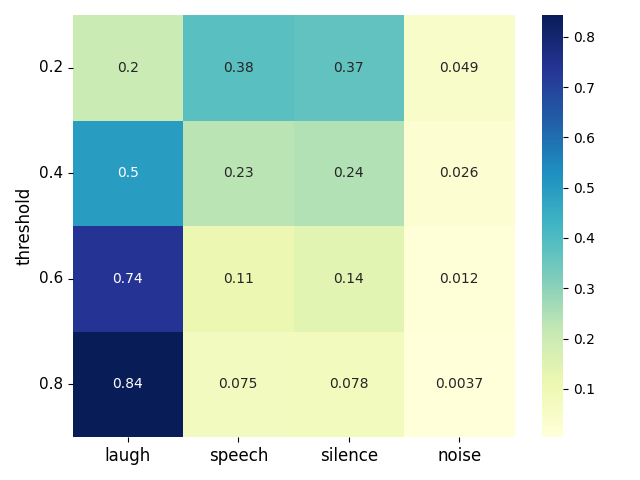
\includegraphics[width=8cm]{imgs/conf_matrix/init_eval_all.png}
    \caption{Example confusion matrix for different thresholds. Each row shows the percentage of laughter segments classified as a certain subclass for a given threshold.}
    \label{fig:example-conf-matrix}
\end{figure}
A confusion matrix is a good way to identify misclassifications. In a multi-class problem, it shows the true label on one axis and the predicted label on the other. It can either show the actual counts of predictions or normalised values between 0 and 1. \autoref{fig:example-conf-matrix} shows a normalised confusion matrix for a classification problem with three classes.
For laughter recognition we only have two classes. Instead of plotting a 2x2 confusion matrix, evaluations in this thesis use a different approach.
Since non-laughter segments can be split into subclasses (as we will see in \autoref{table:segment-types}), we plot the percentage of misclassified laughter samples for each of these classes. 
Each row in \autoref{fig:example-conf-matrix} represents the model outputs for a certain threshold and shows the percentage of laughter samples classified as laughter, speech, silence and noise, respectively. Thus, the sum of all values in a single row is one. 
Note that we cannot get the same diagram for non-laughter segments because the model is a binary classifier. It only predicts laughter and non-laughter but none of the subclasses. 


\chapter{Evaluation of Existing Models for Laughter Detection} \label{cha:model-evaluation}

\section{Model and Data Selection}\label{sec:model-and-data}
After having done the initial research, we decided to focus solely on laughter detection. 
There are two main reasons for this: the type of previous research and open source code available.  
As mentioned in \autoref{cha:bg} most research in the field of laughter and applause detection is done separately. 
Thus, implementing a detection algorithm from existing research requires merging different models. 
For a combined model to work, a good understanding of both domains is essential.
We decided that this is most easily attained by focusing on one domain first. 
We chose to focus on laughter instead of applause because there was an open-source repository available that showcased an existing state-of-the-art laughter detection algorithm \citep{gillick-codebase, gillick2021robust}.

The domain in video conferences is separate single person audio tracks usually recorded in a relatively quiet environment.
To investigate how the existing model might perform in this domain, we decided to evaluate it on the ICSI meeting corpus \citep{morgan2001meeting}. 
We initially considered the use of AudioSet \citep{googleaudioset} as a possible evaluation corpus. We discarded this idea because of a mismatch with the domain of our project. AudioSet  consists of 10s audio segments from Youtube videos which were labeled according to a fixed set of classes - including laughter. Nevertheless, the domain of Youtube videos varies drastically. It contains recordings of someone laughing in a silent environment inside a room and someone laughing in a very noisy environment outside. This variety of environments might help for generalising laughter detection but is not suitable for our project, as we focus on laughter in online meetings.
In contrast, the ICSI corpus is a good match to our domain as it solely consists of meeting speech recorded with both close-distance and table-top microphones. 
We only make use of the close-distance microphone recordings which capture the audio of a single meeting participant.
The ICSI corpus provides transcriptions for all its participants containing speech as well as \texttt{Vocal} and \texttt{NonVocal} tags for sounds like laughter and door squeaks, respectively.
There are two further reasons for using the ICSI corpus: its size and its licence.
The ICSI corpus has a total length of 72h and around 3.9h of total laughter duration suitably transcribed for our use case (\autoref{sec:preprocessing}).
The licence is \href{https://creativecommons.org/licenses/by/4.0/legalcode}{CC BY 4.0} which means that it can be used for commercial projects like an improved version of video meeting software. 


\section{Preprocessing} \label{sec:preprocessing}
Before the model by Gillick et al. can be evaluated on the ICSI corpus, some preprocessing of the corpus data was needed.
At first, the 72 meetings were split into training, development and test set to minimise speaker overlap. The partitioning follows the structure from \citet{renals2014neural}. It uses meetings \texttt{(Bmr021, Bns001)} as development set, meetings \texttt{(Bmr013, Bmr018, Bmr021)} as test set and the remaining 67 meetings as training set.
After this, all laughter segments needed to be filtered out from the raw data to accurately determine correct classifications. 
Lastly, I used the ICSI-transcriptions to divide non-laughter segments into subclasses to get a more rigorous analysis of misclassifications.

\subsection{Filtering out Laughter-only Segments} \label{subsec:filter-laughter}
ICSI transcriptions are split into segments denoted by a start and end time.
Consequently laughter segments co-occurring to speech in one segment cannot be precisely identified.
As mentioned in \autoref{sec:bg-laughter} such data is called weakly labeled.
Strongly labeled data is key for this project because our model should identify laughter segments in a continuous audio stream.
Filtering out strongly labeled laughter segments resembles the approach by \citet{knox2006automatic} to obtain frame-level training data (\autoref{sec:bg-laughter}). 
All weakly labeled segments containing laughter are categorised as invalid and disregarded from the evaluation, a total of 3765 segments.
The remaining 8415 laughter segments have a total duration of 3.9h. \autoref{table:segment-types} shows how this compares to the fraction of other types of audio in the ICSI corpus.

Alternatively, I could have created an ASR model to align weakly-labeled laughter events with their audio counterpart. 
I did not follow this approach due to lack of experience with ASR, which meant that creating such a model would have been time consuming. I considered the 3.9h of pure laughter as sufficient for this project and decided to focus on other parts of the project.
In general, more training data is preferable. Thus, future projects might consider this approach to gain strongly labeled data for the whole corpus and make use of the additional laughter occurrences contained in the invalid segments. 

\begin{table}[h!]
\begin{tabular}{c|c|l}
     subclass & number of segments & total duration \\
     \hline
     laughter & 8415 & 3.9 h \\ 
     invalid & 3765 & 3.7 h \\
     speech & 98418 & 64.1 h \\
     noise & 18224 & 10.9 h \\
     silence & 97431 & 681.9 h 
\end{tabular}
\centering
\caption{Number of segments and total duration of each subclass. Segments can have arbitrary length and are not limited as in \autoref{cha:retraining}.}
\label{table:segment-types}
\end{table}

\subsection{Subclasses of Non-laughter}
In addition to the obvious class division between laughter and non-laughter, we can divide segments into smaller subclasses. This becomes useful when evaluating classification (as we will see in \autoref{cha:experiments}).
For non-laughter segments we can distinguish between speech, invalid segments (as in \autoref{subsec:filter-laughter}), noise and silence.
To summarise, there are five subclasses:
\begin{enumerate}
    \item \textbf{laughter}: segments only containing laughter
    \item \textbf{non-laughter}
    \begin{enumerate}
        \item \textit{speech}: segments only containing speech
        \item \textit{invalid}: segments where laughter occurs together with other sounds (see \autoref{sec:preprocessing})
        \item \textit{noise}: segments containing vocal-sounds like coughing, non-vocal sounds like chair squeaks or a mixture of sounds and speech in one segment
        \item \textit{silence}: segments for which no transcription exists
    \end{enumerate}
\end{enumerate}
Note that these subclasses of non-laughter are not classified by the model. The model is a binary classifier. The distinction within the non-laughter class is merely used for evaluation.
Thus, the confusion-matrices in \autoref{sec:exp1-res} are only for laughter misclassifications as described in \autoref{sec:conf-matrix}.
A breakdown of the amount of each subclass is shown in \autoref{table:segment-types}.


\section{Evaluating Gillick et al's Model on the ICSI Corpus}
In contrast to some existing research \citep{kennedy2004laughter, knox2006automatic} which only used a subset of the ICSI corpus, I evaluated the whole ICSI dataset.
I ran the pre-trained detection model by \citet{gillick2021robust} with four different thresholds for each channel of the 75 meetings - a total of 468 audio tracks. 
Over the course of this project, I corrected the evaluation two times.
The following sections compare the results of these evaluations and provide some analysis on the poor performance of the model.

\subsection{Comparing the Initial and Corrected Evaluations}
In the initial evaluation (\autoref{tab:initial-eval}), the maximum recall achieved was 31.53\%. I expected that a low threshold like 0.2 would yield low precision. Getting such a low recall, however, was surprising. 
\begin{table}[h!]
    \centering
    \begin{tabular}{|c|c|c|}
    \hline
    & \multicolumn{2}{|c|}{initial eval} \\ 
    \hline 
    threshold & precision & recall \\
    \hline
        0.2 &  14.88\% & 31.53\% \\ 
        0.4 &  33.26\% & 17.85\% \\
        0.6 &  49.81\% & 8.05\%  \\
        0.8 &  63.08\% & 3.01\%  \\
     \hline
    \end{tabular}
    \caption{Initial evaluation on 468 audio tracks for different thresholds.}
    \label{tab:initial-eval}
\end{table}



After some discussion, I realised that, even though I filtered out invalid laughter segments from the raw ICSI data as described in \autoref{subsec:filter-laughter}, I did not exclude them from the predictions before evaluation. 
This meant that the model could predict a laughter occurrence correctly but the evaluation method would consider it as false because this laughter occurrence was discarded during preprocessing.
This discrepancy in preprocessing was easily fixed and improved the precision significantly (\autoref{tab:second-eval}). Nevertheless, the recall did not increase by much. 

\begin{table}[h!]
    \centering
    \begin{tabular}{|c|c|c|c|c|}
    \hline
    & \multicolumn{2}{|c|}{initial eval} & \multicolumn{2}{|c|}{considering invalid segs} \\
    \hline 
    threshold & precision & recall & precision & recall \\
    \hline
        0.2 &  14.88\% & 31.53\% & 20.02\% & 37.21\%\\ 
        0.4 &  33.26\% & 17.85\% & 48.39\% & 20.74\%\\ 
        0.6 &  49.81\% & 8.05\% & 73.68\% & 9.14\%  \\ 
        0.8 &  63.08\% & 3.01\% & 91.44\% & 3.33\%  \\ 
     \hline
    \end{tabular}
    \caption{Corrected evaluation considering invalid segments compared with the initial evaluation (\autoref{tab:initial-eval}).}
    \label{tab:second-eval}
\end{table}

Lastly, the final evaluation (\autoref{tab:final-eval}) includes two significant changes: altering the model to remove a filter and introducing a weighted average, as we now explain. 
The evaluation code used by Gillick et al. sometimes yielded probabilities smaller than 0 and larger than 1. 
This bug was caused by a low-pass filter implemented in \verb|laugh_segmenter.py|. I did not investigate this further because neither the code nor the paper stated why this filter was necessary. I fixed the issue by removing the filter.

\begin{table}[h!]
    \centering
    \begin{tabular}{|c|c|c|c|c|c|c|}
    \hline
    & \multicolumn{2}{|c|}{initial eval} & \multicolumn{2}{|c|}{considering invalid segs} & \multicolumn{2}{|c|}{final eval}  \\
    \hline 
    threshold & precision & recall & precision & recall & precision & recall  \\
    \hline
        0.2 &  14.88\% & 31.53\% & 20.02\% & 37.21\%  & 20.86\% & 45.58\%\\
        0.4 &  33.26\% & 17.85\% & 48.39\% & 20.74\%  & 50.26\% & 27.77\%\\
        0.6 &  49.81\% & 8.05\% & 73.68\% & 9.14\%    & 73.77\% & 13.35\% \\
        0.8 &  63.08\% & 3.01\% & 91.44\% & 3.33\%    & 84.53\% & 4.76\% \\
     \hline
    \end{tabular}
    \caption{Final evaluation on 468 audio tracks, compared to the initial (\autoref{tab:initial-eval}) and corrected evaluation (\autoref{tab:second-eval}).}
    \label{tab:final-eval}
\end{table}

Further, introducing a weighted average had a significant impact on the evaluation. The first two evaluations in \autoref{tab:initial-eval} are calculated by averaging the precision and recall of each meeting.
These results can be misleading because meetings vary in duration and some contain significantly more laughter occurrences than others.
\autoref{fig:transc-laughter-distribution} shows that the total duration of laughter occurrences ranges from $<20s$ to $>950s=15min$.
For our use case, it makes sense to take the weighted average because we are interested in the total duration of correctly and incorrectly predicted laughter events, the artificial unit of meetings is an unimportant distinction to us.

To conclude, the final evaluation shown in \autoref{tab:final-eval} should be considered correct and is used as a baseline for further experiments (as we will see in \autoref{cha:experiments}).



\subsection{Analysing Poor Model Performance}

\begin{figure}
    \centering
    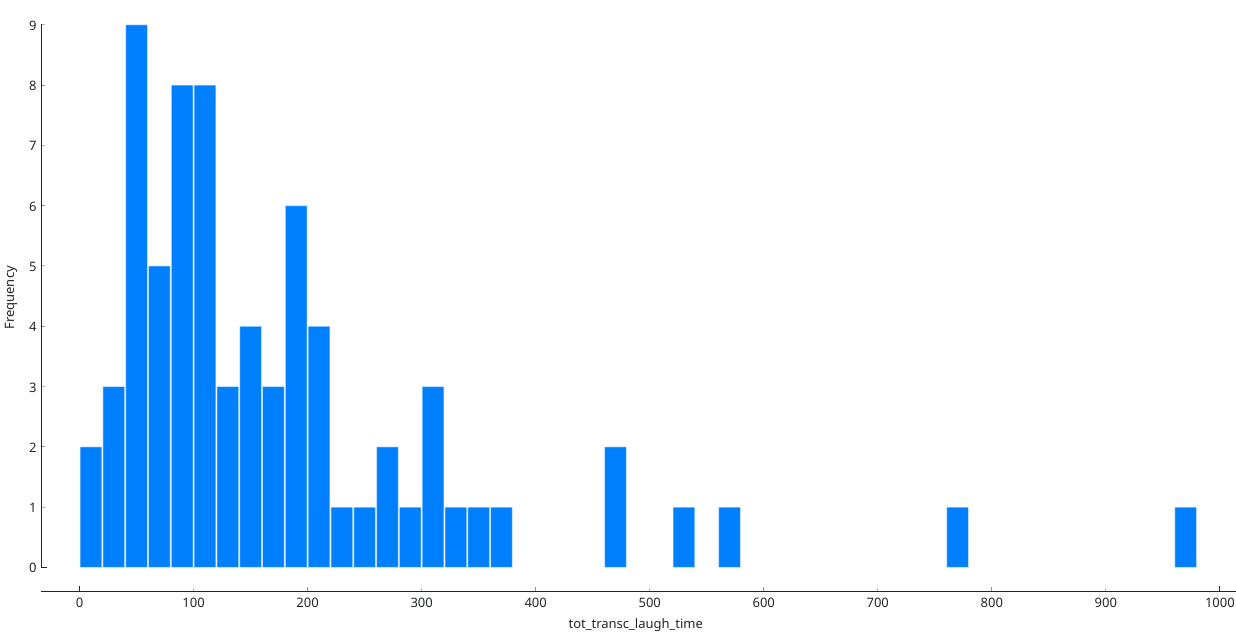
\includegraphics[width=13cm]{imgs/distributions/transcribed_laughter_time_distribution.png}
    \caption{Distribution of transcribed laughter duration per meeting [in s]; bin-width=20s.}
    \label{fig:transc-laughter-distribution}
\end{figure}



To get a better understanding of the performance, \autoref{tab:practical-example} shows what the evaluation would correspond to if this model was implemented as part of a video call system. We assume a meeting that lasts 1 hour and contains a total duration of 4 minutes of laughter. 
Using any of the investigated thresholds would yield an unusable system.
We will briefly examine the two extreme cases. If the threshold was really low, e.g. 0.2, 1:49 min of laughter would be correctly retrieved. Despite this being not even half of the laughter events that occurred we also retrieve almost 7 minutes of noise.  
On the other hand, choosing a high threshold, e.g. 0.8, yields very high precision and thus, only two seconds of noise are transmitted. However, the system merely retrieves 14 seconds of the four minutes of laughter. With such a low percentage of retrieved laughter events, there is no significant difference to participants muting themselves entirely. 

\begin{table}[]
    \centering
    \begin{tabular}{|c|c|c|c|c|c|c|}
      \hline
      threshold & precision & recall & predicted & actual laughter & noise \\
      \hline
      0.2 &  20.86\% & 45.58\% & 8:44 min & 1:49 min & 6:56 min \\
      0.4 &  50.26\% & 27.77\% & 7:16 min & 2:01 min & 5:15 min \\
      0.6 &  73.77\% & 13.35\% & 0:43 min & 0:32 min & 0:11 min \\
      0.8 &  84.53\% & 4.76\% & 0:14 min & 0:12 min & 0:02 min \\
      \hline
    \end{tabular}
    \caption{Practical example using values from the final evaluation \autoref{tab:final-eval}}
    \label{tab:practical-example}
\end{table}


A possible reason for such a bad performance on the ICSI corpus is a data mismatch between training and evaluation data. The pre-trained model by Gillick et al. \citep{gillick2021robust} was trained on the Switchboard corpus \citep{switchboard-corpus}. The Switchboard corpus records telephone conversations between two participants at a sample rate of 8000hz. The ICSI corpus records meeting speech of multiple participants at a sample rate of 16000hz. For prediction, all audio tracks are down-sampled to 8000hz which results in losing lots of the original data. 
Further, the Switchboard dataset has one audio track containing the audio from both participants whereas the ICSI corpus has separate audio tracks for each participant. Thus, especially the long periods of silence on each individual channel are new to the model. 

\begin{figure}[h!]
    \centering
    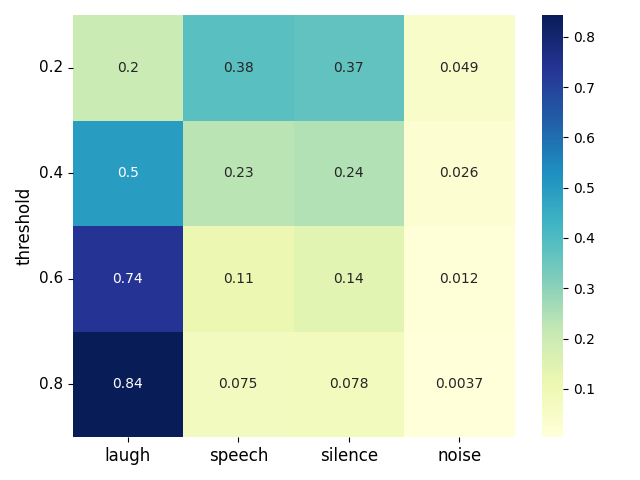
\includegraphics[width=8cm]{imgs/conf_matrix/init_eval_all.png}
    \caption{Confusion matrix for final evaluation (\autoref{tab:final-eval}), evaluated on the whole ICSI corpus. \confmatrixcaption}
    \label{fig:initial-conf-matrix}
\end{figure}

Looking at the confusion matrix in (\autoref{fig:initial-conf-matrix}) we notice that misclassifications are almost evenly split between silence and speech regions. This is surprising because I expected silence to be easier to distinguish from laughter than speech.
Further evaluation and insights also referring back to this initial evaluation can be found in \autoref{cha:experiments}.
In response to this finding, I decided to retrain the model on the ICSI corpus. 


\chapter{Training Laughter Detection on the ICSI Corpus} \label{cha:retraining}
\section{Adapting Gillick et al's Training Code} 
The first approach was to adapt Gillick et al.'s published code \citep{gillick-codebase}, which used PyTorch \citep{pytorch2017automatic}, an open-source machine learning framework for python.
Parts of the code were cumbersome and disregarded current standards of PyTorch programs, e.g. they used a manual batch counter for training steps instead of using epochs.  

Despite these concerns, I decided to adapt their existing code for two reasons.
Firstly, developing the whole framework from scratch would have been time consuming and slightly precarius as I had never worked on a machine learning project of this scale.
%Thus, I considered it safer to use Gillick et al's code, as it is the foundation of a published paper from Interspeech 2021 \citep{gillick2021robust}. 
Secondly, slightly adjusting the code allows for an comparison between the original and retrained model. 

\autoref{fig:gillick-data-pipeline} shows the data-pipeline used by Gillick et al. The raw inputs per conversation are one audio track and two transcription files. 
Firstly, all audio tracks are preloaded into memory, serialised and stored as a hash-map. Every time the model is trained the hash-map is loaded into memory to minimise disk accesses which slow down the training. 
Secondly, Gillick et al. filter out all laughter segments and store them in a table as shown in \autoref{fig:gillick-data-pipeline}.
They add the same amount of non-laughter segments to this dataframe. 
Note that tables are also referred to as dataframes in this thesis; this term originates from the commonly used data-analysis python library pandas \citep{jeff_reback_2021_5574486}.
Each segment is stored with its start-time, duration, subsample start-time, subsample duration, audio path and label where 1 means laughter and 0 means non-laughter. 
This dataframe and the hash-map are the inputs for a PyTorch Dataset. This dataset defines the data structure for the PyTorch DataLoader which is used to sample batches during training.

\begin{figure}
    \centering
    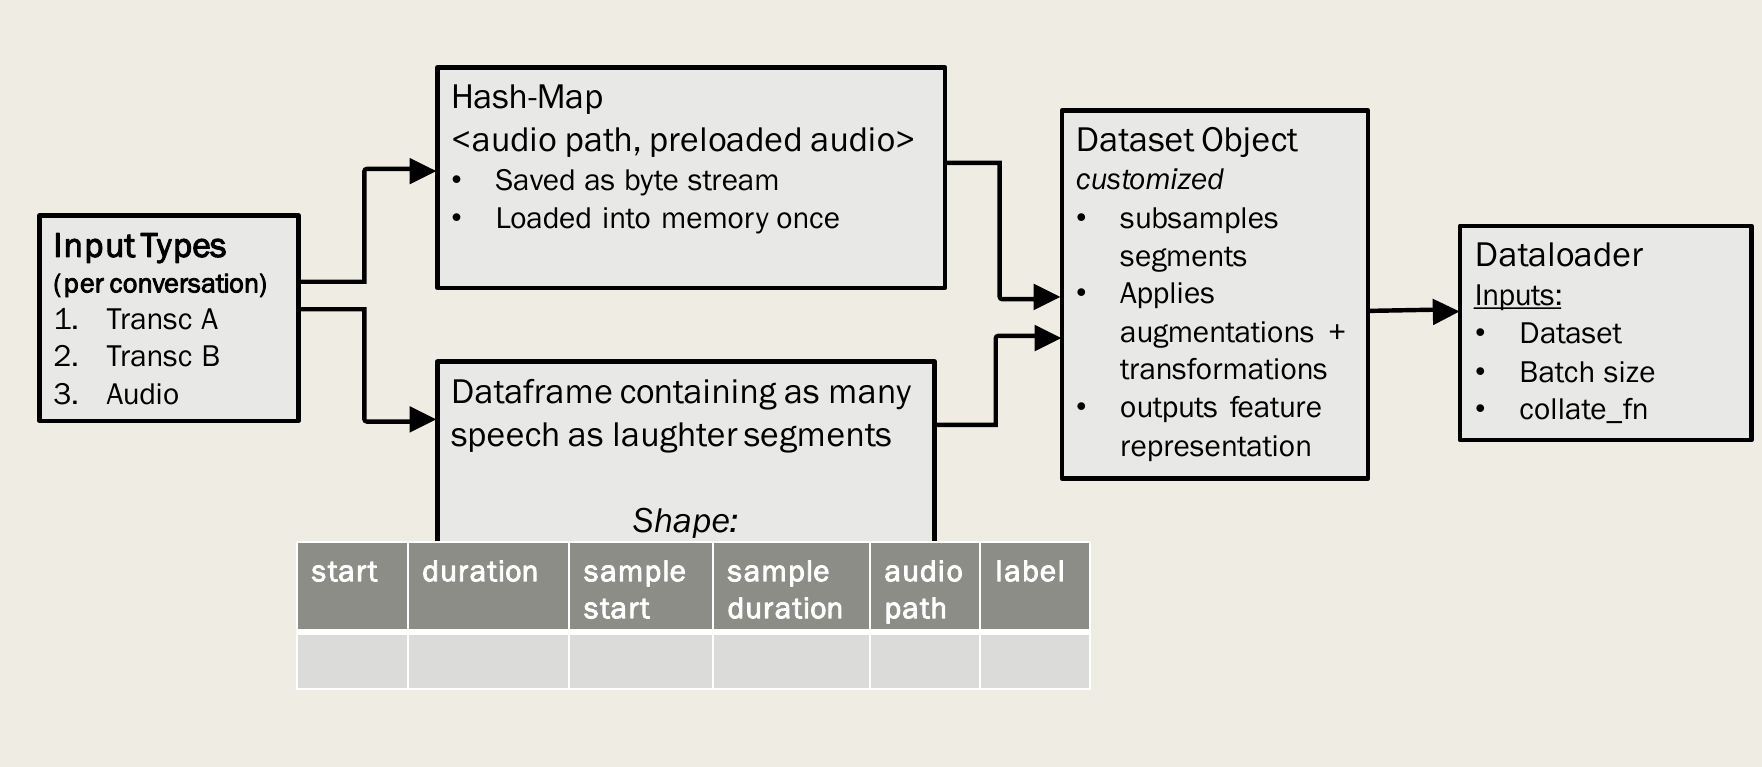
\includegraphics[width=14cm]{imgs/diagrams/Gillick_et_al_data_pipeline.png}
    \caption{Data pipeline used by \citet{gillick2021robust}. I created this pipeline based on Gillick et al's code \citep{gillick-codebase}. This diagram was not part of the original paper.}
    \label{fig:gillick-data-pipeline}
\end{figure}

Creating a hash-map with serialised audio data from the ICSI corpus failed due to missing memory. Since the ICSI corpus contains single audio tracks for each participant the total size is larger than the Switchboard dataset. In addition, the sample rate is twice as high. 

The following estimates show the difference in storage space needed to preload the whole ICSI/Switchboard corpus as .wav-files. We assume a bit rate of $16bits=2bytes$ per sample.

The Switchboard corpus consists of 260 hours of raw audio sampled at 8khz which can be estimated as:

$$ \frac{260\;\textrm{hours} \cdot 3600\;\textrm{seconds} \cdot 8000\;\textrm{samples per second} \cdot 2\;\textrm{bytes}}{1024^3} \approx 13.95 GB $$  

The ICSI corpus contains 72hours of meeting speech with an average of six participants per meeting. Thus, there are 72*6=432 hours of audio sampled at 16khz:

$$ \frac{432\;\textrm{hours} \cdot 3600\;\textrm{seconds} \cdot 16000 \;\textrm{samples per seconds} \cdot 2bytes}{1024^3} \approx 46.35 GB $$

Using a machine with sufficient RAM would allow loading the whole audio data into memory. 
Regardless of missing access to such a machine finding a solution that requires less RAM is desirable. Thus, I decided to rewrite the DataLoader from scratch. 

The first version of this DataLoader resulted in slow training. The model trained around 30 batches of audio in two hours, each consisting of 32 audio tracks. 
With training samples of one second each, this equates to one sample every eight seconds.
This training performance on a GPU machine was significantly worse than the inference performance on a CPU-only machine (\autoref{tab:rtf}).

The GPU was not used most of the time because the data-loading was the bottleneck. In contrast to inference, where an audio track is loaded at the beginning, training required the DataLoader to load many one-second segments from different. 
Without any pre-loading in place, the segments were loaded on-the-fly, requiring one disk access per one-second segment. This meant the GPU was starved, i.e. waited for input most of the time. 
In addition, loading data from large offsets using the librosa library \citep{mcfee2015librosa}, a popular python library for audio analysis, was significantly slower than loading data from the beginning of an audio file. A crude analysis (\autoref{tab:librosa-loading-times}) shows that the loading time grows with the offset at which this sample is located. 
This is especially problematic because ICIS's average meeting length of 58 minutes \citep{icsi-ldc} is significantly longer than the 6.5 minutes for Switchboard recordings \citep{switchboard-ldc}.
I later realised that this problem only arose because ICSI audio-files are stored as \verb|.sph|-files. Converting all files to \verb|.wav|-files could have solved this issue, but the main bottleneck would have persisted, namely the large number of disk accesses due to on-the-fly data-loading.

\begin{table}[h!]
    \centering
    \begin{tabular}{|c|c|c|c|}
    \hline
    offset[s] & average time[s] & total time[s] & iterations run \\
    \hline
    0  & 0.15 & 4.40 & 30    \\
    300 & 0.34 & 10.16 & 30  \\ 
    700 & 0.59 & 17.72 & 30  \\
    1000 & 0.78 & 23.36 & 30 \\  
    3000 & 2.03 & 60.79 & 30 \\
    5000 & 3.26 & 97.65 & 30 \\
    \hline
    \end{tabular}
    \caption{Using librosa \citep{mcfee2015librosa} to load a one-second segment from different offsets of an audio-file. Channel loaded: \texttt{Btr002:chan3}. Duration: 5318s. Test code: \href{https://github.com/LasseWolter/laughter-detection-icsi/tree/main/misc_scripts}{naive librosa-test}.}
    \label{tab:librosa-loading-times}
\end{table}


My second supervisor suggested the use of Lhotse \citep{zelasko2021lhotse} to speed up the data-loading. Lhotse is a currently developed python library for speech and audio data preparation which is already usable.

\section{A Data Pipeline Using Lhotse}
This section outlines how I used Lhotse to recreate the data pipeline to speed up data-loading. I first give a brief introduction into Lhotse and why it is suitable for our use case. Then I explain some necessary adjustments and finally present my data-pipeline which is part of the published \coderepo.

\subsection{Lhotse} \label{sec:lhotse}
Two main features make Lhotse suitable for my use case:
\begin{enumerate}
    \item Simplified loading of popular corpora like ICSI
    \item Sample creation without actually loading audio data from disk
\end{enumerate}

Lhotse provides so-called \textit{recipes} which simplify working with popular corpora like the ICSI corpus.
These \textit{recipes} are python scripts that create \textit{manifests}.
\textit{Manifests} are representations of the entire corpus only containing meta data of the recordings as well as the corresponding supervisions, i.e. transcriptions.
Using those manifests Lhotse creates samples - called \textit{Cuts} in Lhotse - without loading audio or transcript data into memory. 

Due to Lhotse being in development I made some adjustments. The \textit{recipe} for the ICSI corpus was not part of the latest release \textit{v0.12} which meant that I had to work with the development version. 
I fixed some bugs in the ICSI \textit{recipe}. 
I ran into some other issues with Lhotse and decided to debug some of them. Despite some of the debugging was not strictly necessary for my project, I decided to contribute to this open source project which has the potential to be useful in the field of audio and speech processing in the future. A list of my contributions, containing links to the corresponding pull requests can be found in \autoref{app:lhotse-contrib}. All contributions have been accepted and are now part of the Lhotse library.

\subsection{Data Pipeline} \label{sec:ml-data-pipeline}

\autoref{fig:data-pipeline} shows the data pipeline.
Initially, Lhotse's \textit{ICSI-recipe} takes the raw data and creates a manifest representing the ICSI corpus (\autoref{sec:lhotse}).
Besides this manifest creation there are two main functions in the data pipeline: \verb|create_data_df| and \verb|compute_features|. 
\verb|compute_features| has two parts.

The first part of \verb|compute_features| uses the ICSI-manifest to create a feature representation of all audio tracks in the corpus. Following standards in the ASR community, mel spectrogram features of shape 100x40 are used (\autoref{fig:feature-sample}). The impact of different feature representations is further discussed in \autoref{sec:real-time}. 
Manifest creation and feature computation for the whole corpus, marked in blue, only need to happen once.
Note that if the feature representation is changed, this part of \verb|compute_features| needs to be run again to update the features of the whole corpus.


\begin{figure}[h!]
    \centering
    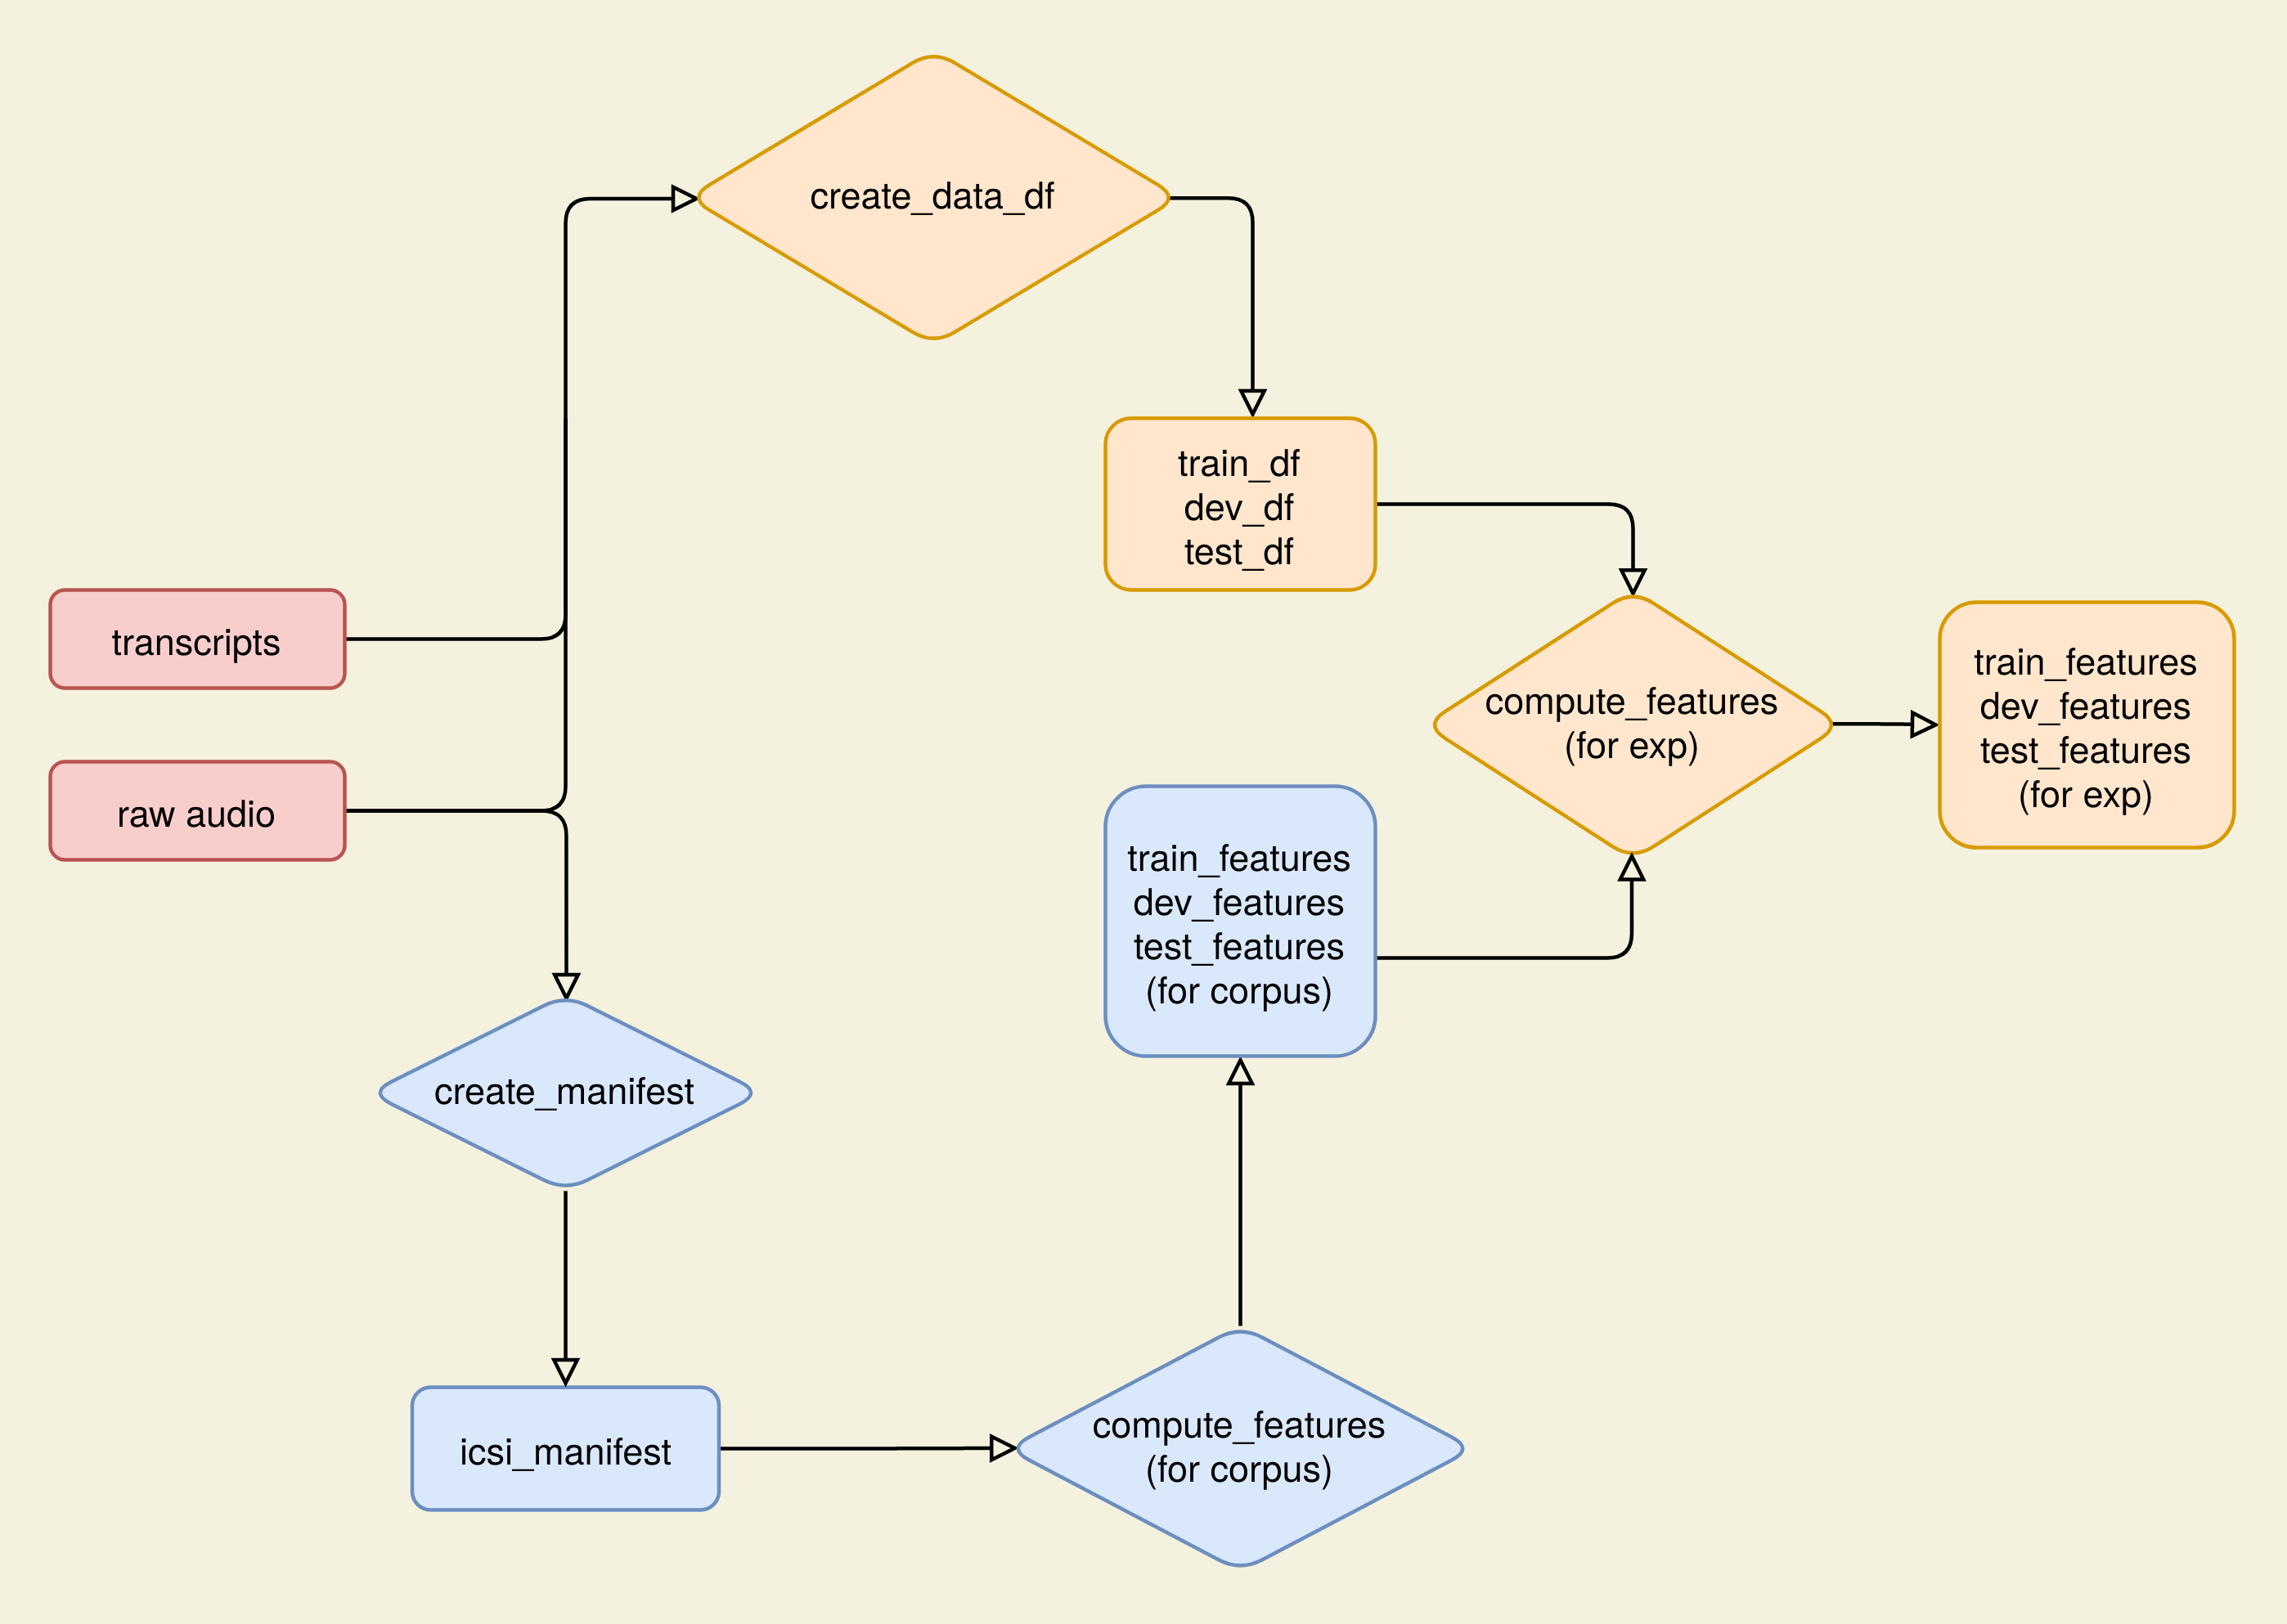
\includegraphics[width=15cm]{imgs/diagrams/Pipeline.drawio.png}
    \caption{Data Pipeline. Rectangles represent data, diamonds represent functions. The arrows show input and output of these functions. \texttt{df} stands for dataframe.}
    \label{fig:data-pipeline}
\end{figure}

The remaining parts, marked in orange, need to be run every time the model is trained on a new subset of the corpus.
\verb|create_data_df| creates the three dataframes of the shape shown in \autoref{fig:gillick-data-pipeline}, one for each split.
These dataframes are then input into the second part of the \verb|compute_features| function which take the feature representation of the whole corpus and extract the parts defined in the corresponding dataframe. This is guaranteed to be fast because no features are computed at this stage.
We end up with three sets of features, one for each split. 
These feature are loaded during training time which means that no raw audio or feature computation needs to happen during training itself.

\begin{figure}[h!]
    \centering
    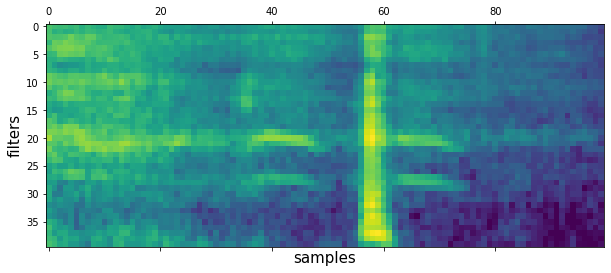
\includegraphics[width=14cm]{imgs/sample_fbank_feat.png}
    \caption{Example feature representation of a 1s laughter segment}
    \label{fig:feature-sample}
\end{figure}

\href{https://github.com/LasseWolter/laughter-detection-icsi/blob/main/Demo.ipynb}{This jupyter notebook} demonstrates a simplified version of how \verb|compute_features.py| computes features. 
The main difference is that the provided example loads the audio file directly into a Lhotse Cut whereas \verb|compute_features.py| loads already computed feature representation of the whole meeting and only selects the requested subset. In practice, this is a lot faster for computing large amounts of features.

I did not make use of the automatically created supervisions by the \textit{ICSI-recipe} because I already created the \verb|create_data_df| function at an earlier stage and considered reusing it the easier approach.
The generated dataframes contained all information needed for a supervision segment: the channel, the start and end time of a segment as well as its label. 
I adapted a PyTorch Dataset\footnote{Dataset here does not refer to actual data. It refers to one of the two main PyTorch primitives for data handling: \href{https://PyTorch.org/tutorials/beginner/basics/data_tutorial.html}{Datasets}} for \href{https://lhotse.readthedocs.io/en/latest/datasets.html#lhotse.dataset.vad.VadDataset}{voice activity detection} already provided by Lhotse.
For future work using the supervision segments provided by Lhotse can simplify the pipeline even further by making the \verb|create_data_df| function obsolete. 

\section{Training}
Given the data-pipeline outlined in \autoref{sec:ml-data-pipeline} the actual training was straightforward. For each different subset of the corpus I needed to rerun the \verb|create_data_df| and \verb|compute_feature| functions to create the features. 
These features were loaded into the modified VAD Dataset which I called LAD: laugh activity detection.
During training time, data is extracted from this dataset using the texttt{SimpleCutSampler} provided by Lhotse. 
This new approach can process 44000 batches in 2 hours compared to the 30 batches of my initial training approach which allows for high training speed without having to load all the raw audio into memory.
To allow for direct comparisons, I used the same ResNet architecture as \citet{gillick2021robust}.
The performance of this model trained on different subsets of the ICSI corpus is investigated in the next section.

\chapter{Investigating the Impact of Training Data on Model Performance} \label{cha:experiments}
Representative training data is essential for machine learning. Training on the whole ICSI corpus would take a long time and was not feasible for my project.
Thus, the following experiments investigate how the selection of a corpus-subset for training impacts the model's performance. 
Due to significant time spent on task already outlined in the thesis, the following experiments do not include exhaustive grid searches. Hence, the results of these experiments should be considered as pointers for future research, not an optimal solution.

The structure of training data was investigated in two dimensions: 
\begin{enumerate}
    \item class balance between laughter and non-laughter samples
    \item diversity of non-laughter samples 
\end{enumerate}

All evaluations in this section are done on the development set of the ICSI corpus as defined in \autoref{sec:preprocessing}.

\section{Experiment 1 - Class Balance} \label{sec:exp-1}
In the first set of experiments evaluates different ratios between laughter and non-laughter segments in the training data.
Three different ratios between laughter and non-laughter segments are compared with the pre-trained model by \citet{gillick2021robust}: 1-to-1, 1-to-10 and 1-to-20.
The sample duration is one second, as also used by \citet{gillick2021robust}. The feature shape differs from the pre-trained model. \citet{gillick2021robust} use mel spectrograms of shape 44x128 whereas the newly trained models uses a shape of 100x44.
Further, neither subsampling nor feature augmentation was applied during training which helped \citet{gillick2021robust} to achieve minor performance improvements.
I initially planned to investigate these three dimensions further: feature shape, subsampling and feature augmentation. 
Due to time constraint I did not conduct such experiments, which leaves this task for future work. 

The non-laughter segments are sampled at random from all non-laughter segments, without considering the subclass. 
\autoref{sec:exp2} investigates a fixed distribution between these subclasses. 

% The non-laughter segments were selected on a random basis from the remaining audio tracks after subtracting the laughter and invalid regions (\autoref{table:segment-types}). 

\subsection{Method}
To select non-laughter segments across a variety of meetings, \verb|create_data_df| uses the following selection process.
For each laughter segment, a channel within the same meeting is selected at random.
A non-laughter segment of the same duration as the laughter segment is sampled from this channel.
If the laughter segment is longer than one second, both laughter and non-laughter segments are truncated to a random one-second region of their segment. 
If the segment is shorter than one second, it is stored unmodified and padded to one second length during feature computation.
All these segments are stored in a table as explained in \autoref{sec:ml-data-pipeline}.
In contrast to random sampling across all meeting, this approach guarantees that the training data holds non-laughter segments from all meetings containing laughter. 

\subsection{Results} \label{sec:exp1-res}

\begin{figure}[h!]
    \centering
    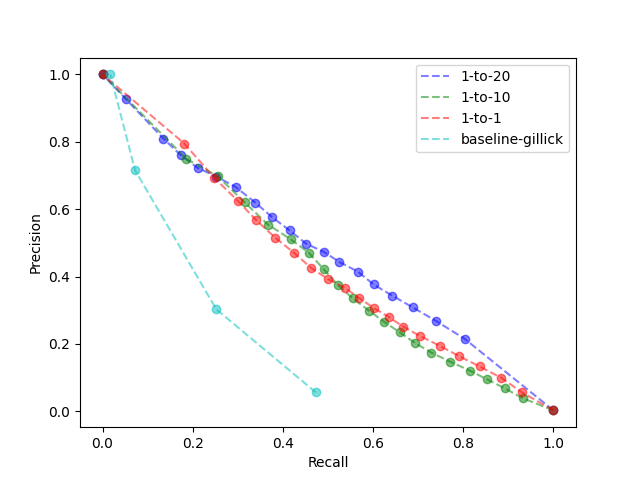
\includegraphics[width = 3.8in]{imgs/prec-recall/exp1-random/dev_compare_class_balance_dev_set.png}
    \caption{Precision-Recall-Curve for different ratios between laughter and non-laughter based on 21 evenly spaced thresholds from 0 to 1.  The baseline, given by the model from \citet{gillick2021robust} evaluated the development set, only has four data points for thresholds [0.2,0.4,0.6,0.8], because it uses the initial evaluation from \autoref{cha:model-evaluation}.}
    \label{fig:prec-recall-rand}
\end{figure}

\autoref{fig:prec-recall-rand} compares the performance of the newly trained models with the baseline, the pre-trained model by \citet{gillick2021robust} evaluated on the development set.
The data points displayed in \autoref{fig:prec-recall-rand} are precision and recall for 21 evenly spaced thresholds from 0 to 1.
All models trained on the ICSI corpus outperform the baseline.
Overall there is little differences between the three new models, but for $mathtt{recall} > 0.3$ the 1-to-20 model performs best. 

\autoref{fig:conf-matrix-rand} shows a confusion matrix for different thresholds to deepen the understanding of the misclassified laughter samples. Note that the baseline is not same confusion matrix as \autoref{fig:initial-conf-matrix} because this time we only evaluate on the development set.
For all newly trained models most misclassifications are in silence regions, regions that have no transcription. 
In contrast, the baseline classifies more laughter samples as speech than silence. Generally, we note that there is only a small amount of samples located in noise regions, the baseline has almost none.
The 1-to-20 model has the least speech samples across all thresholds, except for threshold 0.8 where the baseline has 100\% precision, i.e. all predicted laughter samples are indeed laughter samples.


\begin{figure}[h!]
\begin{tabular}{cc}
\hspace*{-2cm}                                                           
\subfloat[1-to-20]{\includegraphics[width = 3.5in]{imgs/conf_matrix/exp1-random/1_to_20_random.png}} &
\hspace*{-1cm}                                                           
\subfloat[1-to-10]{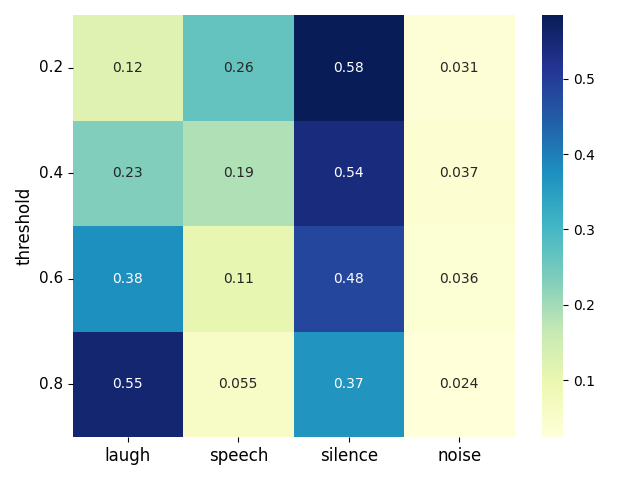
\includegraphics[width = 3.5in]{imgs/conf_matrix/exp1-random/1_to_10_random.png}}\\ 
\hspace*{-2cm}                                                           
\subfloat[1-to-1]{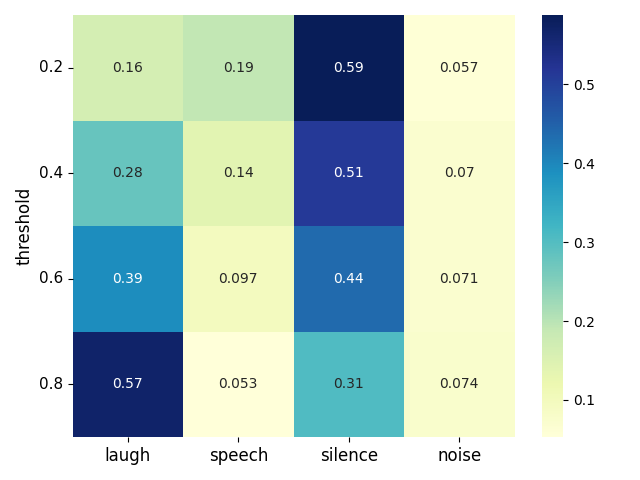
\includegraphics[width = 3.5in]{imgs/conf_matrix/exp1-random/1_to_1_random.png}} &
\hspace*{-1cm}                                                           
\subfloat[baseline-gillick]{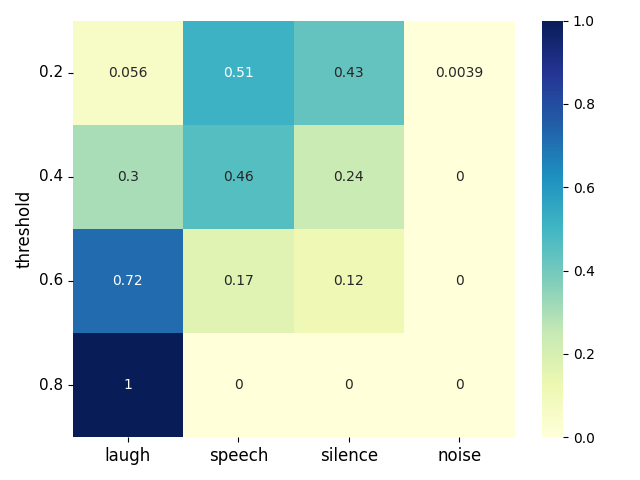
\includegraphics[width = 3.5in]{imgs/conf_matrix/exp1-random/baseline.png}}\\ 
\end{tabular}
\caption{Confusion matrices for different ratios between laughter and non-laughter. \confmatrixcaption Baseline is given by the model from \citet{gillick2021robust} evaluated on the development set (note: \autoref{fig:initial-conf-matrix} was evaluated on the whole ICSI corpus).}
\label{fig:conf-matrix-rand}
\end{figure}

\subsection{Analysis} 
The purpose of the experiment was to investigate different class balances. 
The precision-recall curve (\autoref{fig:prec-recall-struc}) suggests that the 1-to-20 ratio gives the best performance, even though put into context, the performance is still poor. 
All three models trained on the ICSI perform significantly better than the baseline from \citet{gillick2021robust} which was trained on the Switchboard dataset (as in \autoref{cha:model-evaluation}).
This behaviour is expected and aligns with findings from \citet{gillick2021robust} (\autoref{fig:gillick-results}). A model evaluated on the same dataset it was trained on performs better than a model trained on a different dataset. 

Another insight is deduced from the confusion matrices. Whereas the baseline has more misclassified speech than silence segments, the three newly trained models misclassify speech less often. 
In contrast, the newly trained models often misclassify silence regions, regions with no transcription, as laughter.
Evaluating the pre-trained model by \citet{gillick2021robust} on the whole ICSI corpus (\autoref{cha:model-evaluation}) showed a non negligible amount of misclassifications in silence regions. 
These newly trained models make this problem even more apparent and raise the question, why the model is not able to confidently separate laughter from silence.
Lastly, the 100\% precision of the pre-trained model for a threshold of 0.8 should be seen in context. A precision of 100\% alone does not mean a good model performance as described in \autoref{sec:acc-prec-rec}. Looking at \autoref{fig:prec-recall-rand}, this threshold corresponds to the light blue data point in the top left corner. This shows that this threshold is close to one extreme of the precision recall curve where precision is 100\% and recall is 0\%. Future work could investigate why the pre-trained model already reaches this extreme at a threshold of 0.8, but compared to other future tasks I consider this as less important.

\section{Experiment 2 - Non-laughter Diversity} \label{sec:exp2}
The second set of experiments investigates the impact of the different types of non-laughter on the model performance. 
Thus, the ratio of non-laughter segments was fixed to 1-to-20. The ratio 1-to-20 was chosen to maximise the amount of non-laughter segments and be able to use one of models from \autoref{sec:exp-1} as a baseline.
The segment selection and feature computation process was similar, but non-laughter segments were not chosen at random. A fixed percentage of non-laughter segments was assigned to each of the three types of non-laughter: speech, noise and silence.
\autoref{tab:exp-2-subclass-split} shows the different percentages tried.

\begin{table}[h!]
    \centering
    \begin{tabular}{|c|c|c|c|c|}
        \hline
        model & speech & silence & noise \\
        \hline
        a &  70\% & 10\% & 20\% \\
        b &  10\%  & 70\% &  20\%\\
        c &  20\%  & 70\% & 10\% \\ 
        \hline
    \end{tabular}
    \caption{Percentages of non-laughter subclasses for experiment 2.}
    \label{tab:exp-2-subclass-split}
\end{table}

\subsection{Results}
\begin{figure}[h!]
    \centering
    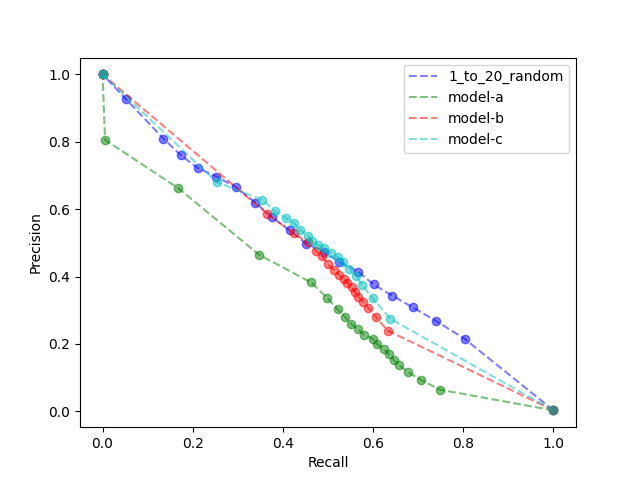
\includegraphics[width = 3.8in]{imgs/prec-recall/exp2-structured/dev_compare_class_balance_dev_set.png}
    \caption{Precision-Recall-Curve for different splits of non-laughter subclasses as shown in \autoref{tab:exp-2-subclass-split}. Baseline taken from experiment one (\autoref{sec:exp-1}) where non-laughter segments were sampled randomly.}
    \label{fig:prec-recall-struc}
\end{figure}


\begin{figure}[h!]
\begin{tabular}{cc}
\hspace*{-2cm}                                                           
\subfloat[model-a]{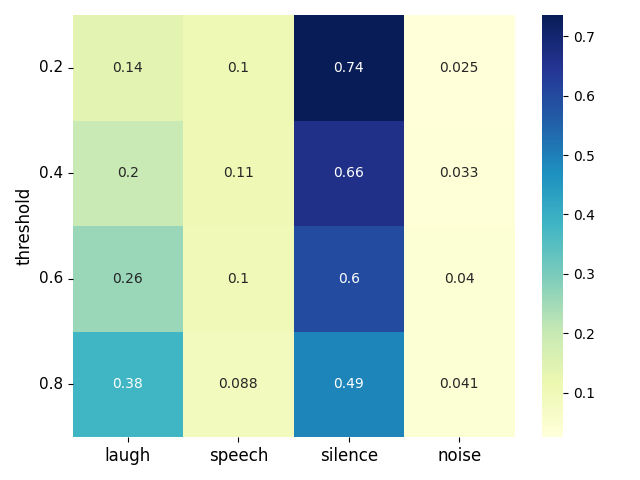
\includegraphics[width = 3.5in]{imgs/conf_matrix/exp2-structured/model-a.png}} &
\hspace*{-1cm}                                                           
\subfloat[model-b]{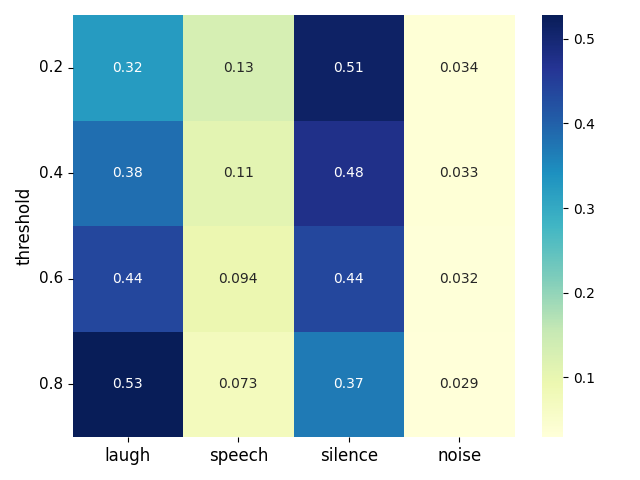
\includegraphics[width = 3.5in]{imgs/conf_matrix/exp2-structured/model-b.png}}\\ 
\hspace*{-2cm}                                                           
\subfloat[model-c]{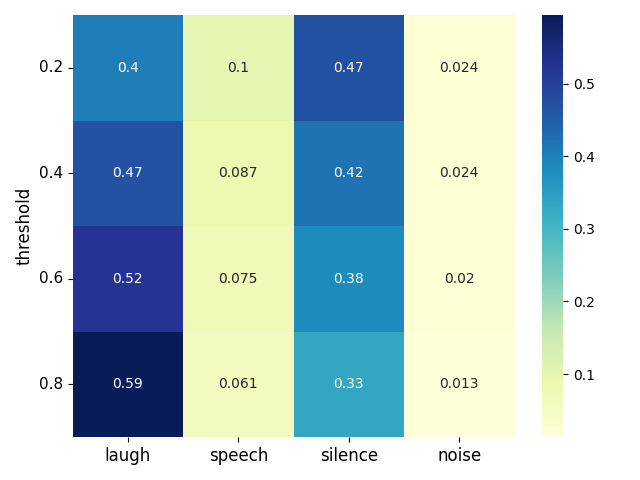
\includegraphics[width = 3.5in]{imgs/conf_matrix/exp2-structured/model-c.png}} &
\hspace*{-1cm}                                                           
\subfloat[baseline]{\includegraphics[width = 3.5in]{imgs/conf_matrix/exp2-structured/1_to_20_random.png}}\\ 
\end{tabular}
\caption{Confusion matrices for different splits of non-laughter types as shown in \autoref{tab:exp-2-subclass-split}. \confmatrixcaption}
\label{fig:conf-matrix-struc}
\end{figure}

Looking at the precision-recall curve in \autoref{fig:prec-recall-struc}, we see that \texttt{model-a} performs worse than the baseline. \texttt{model-c} performs similar to the baseline with worse performance in the area of $recall > 60\%$. \texttt{model-b} performs slightly better for the area $0.3<recall<0.6$, but worse for recalls higher than this.
We note that the majority of data points for \texttt{model-b} and \texttt{model-c} are condensed in the area of $0.3 < recall < 0.7$ and $0.1 < precision < 0.6$.

\autoref{fig:conf-matrix-struc} compares the confusion matrices. The general structure is similar to the matrices in \autoref{fig:conf-matrix-rand}.
Most of the misclassifications are silence segments. 
The proximity of adjacent data points visible in the precision-recall curve becomes evident in the matrices as well. Laughter percentages for the displayed thresholds are low. 
Further, the bright colours in the speech column matrix for \texttt{model-a} show that it retrieves a lot of speech samples. 
Lastly, we can see that \texttt{model-c} has slightly more speech misclassifications than the other three models.


\subsection{Analysis}
The goal of these experiments was to analyse the impact of diversity within the non-laughter segments. Using only a few silence segments decreases model performance significantly.
The impact of slightly changing amounts of noise, speech and laughter but keeping the number of silence segments constant yielded a small performance impact. 
Thus, only considering this set of experiments, changing the number of silence segments in the non-laughter class has the most impact. 
This is not a definitive conclusion but merely a result of this small set of experiments. 
The confusion matrices in \autoref{fig:conf-matrix-struc} do not add much to the insights from experiment 1 (\autoref{sec:exp-1}). The higher number of misclassified speech segments in \texttt{model-c} should be noted but cannot be put into context with other observations.

\section{Investigating Non-transcribed Regions in the ICSI Corpus} \label{sec:silence-regions}
Both, the initial evaluation (\autoref{cha:model-evaluation}) and the experiments (\autoref{cha:experiments}) raised the question, why the model is not able to separate laughter from silence segments in the corpus. Thus, I decided to manually analyse some audio tracks for abnormalities. This is a crude analysis to come up with a hypothesis for the large amount of retrieved silence segments.

I randomly selected five of the 468 audio tracks and plotted their audio-wave (\autoref{fig:rand-audio-track}). The selected tracks are plotted in this order:
\begin{enumerate}
    \item Bmr027: chan5
    \item Bdb001: chan4
    \item Btr001: chan7
    \item Bns003: chan0
    \item Bmr018: chan1
\end{enumerate}

\begin{figure}[h!]
    \centering
    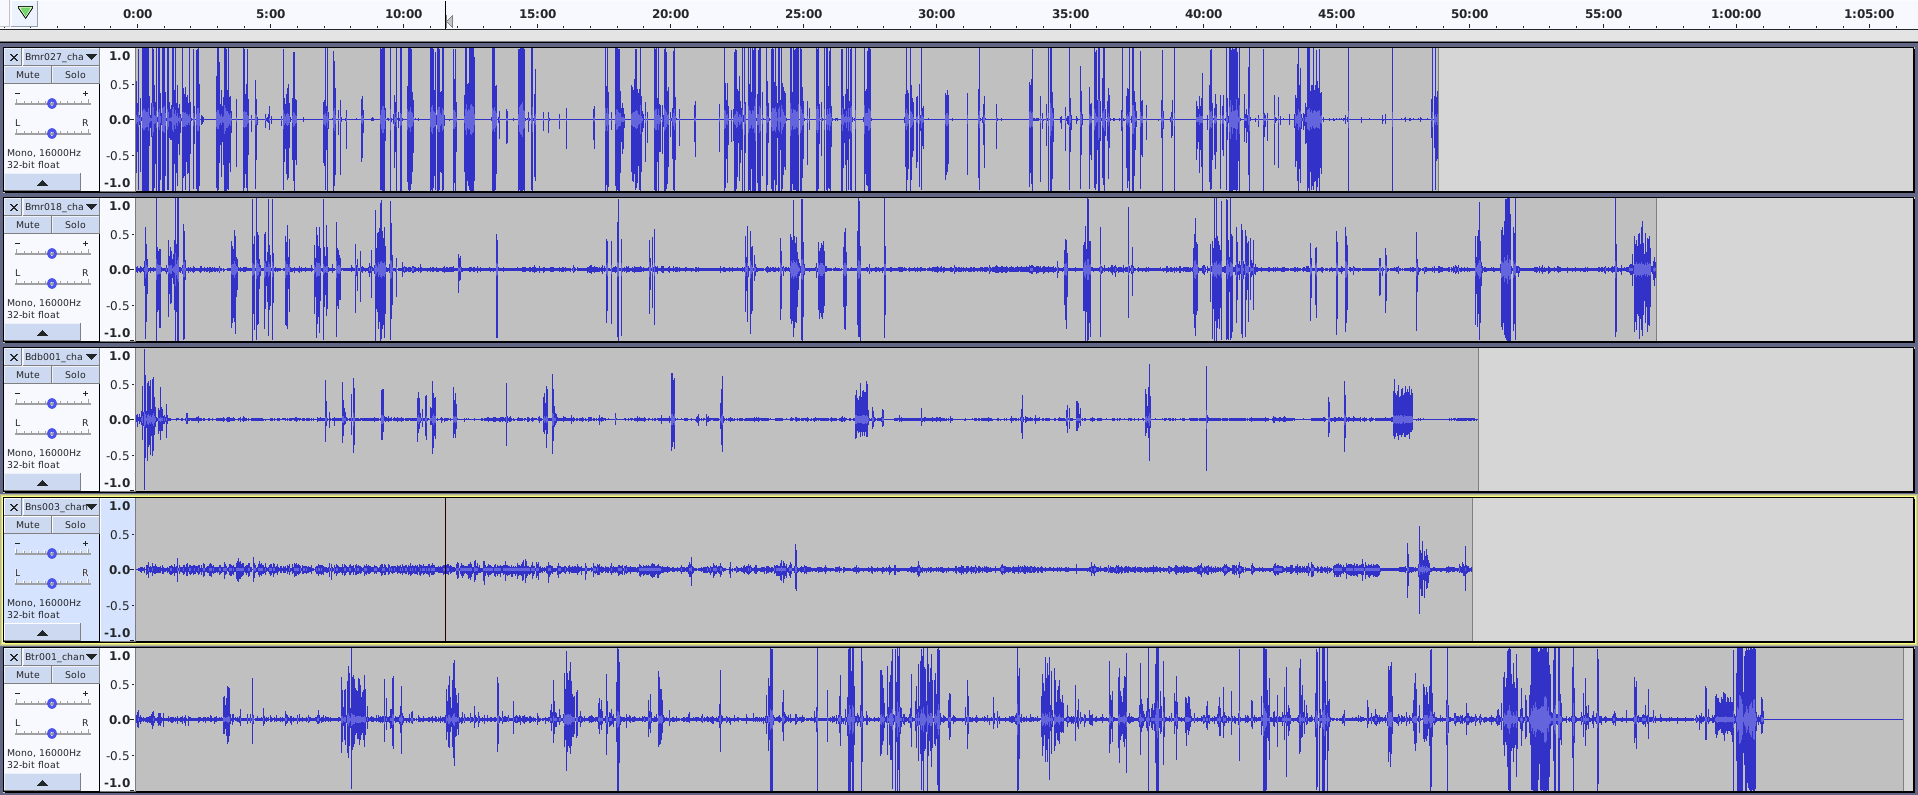
\includegraphics[width=14cm]{imgs/audio_waves/plotted_audio_waves.png}
    \caption{Audio waves of five random audio tracks from the ICSI corpus}
    \label{fig:rand-audio-track}
\end{figure}

\begin{figure}
    \centering
    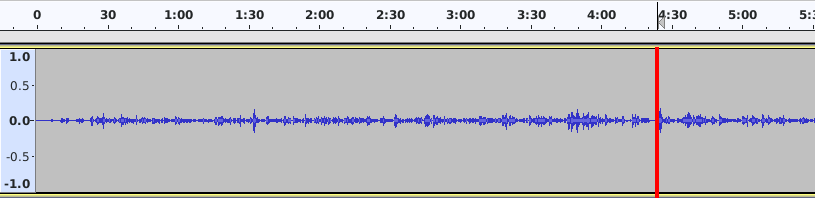
\includegraphics[width=12cm]{imgs/audio_waves/Bns003_cha0_first_transcribed_occurence.png}
    \caption{\texttt{Bns001:chan0}. First transcribed occurrence marked by red line. Considering transcriptions, everything else should be silence. This is not visible in the audio wave.}
    \label{fig:bns001-chan0-audio-wave}
\end{figure}
Depending on the activity and looking at the corresponding transcript I listened to segments of the recordings that were supposed to be silent. In all cases, except for \verb|Bmr027:chan5|, I was able to clearly hear the other participants speaking. 
\verb|Bmr027:chan5| (the top recording in \autoref{fig:rand-audio-track}) was recorded with a different headset than the other four tracks which is likely the reason why there is actual silence on this track.
\verb|Bns003:chan0| (fourth row in \autoref{fig:rand-audio-track}) is the most problematic. There is almost no difference between the volume of the participant speaking to the rest of the meeting. \autoref{fig:bns001-chan0-audio-wave} shows the first transcribed occurrence, a short laughter, which is not distinguishable from the rest of the audio wave.

From this analysis, I conclude the falsity of the assumption that everything not transcribed is silence. Thus, the areas classified as silence in the preprocessing (\ref{sec:preprocessing}) are not actually silence for a significant number of cases; they are quieter recordings of speech by other participants. 
In hindsight, such an analysis at an earlier stage of the project would have prevented false assumptions. 

Future work should further investigate the non-transcribed regions and explore methods to deal with them.
One approach could be to examine all channels recorded with the headset type used by channel \verb|Bmr027:chan5|, tagged with \texttt{c1} in the ICSI transcriptions \citep{morgan2001meeting, icsi-naming-conventions}. If all of these recordings proof to be of higher quality in terms of separating activity from silence, only evaluating on those channels could reveal if noise within non-transcribed regions is the issue.

Another approach would be to filter for meetings with little volume variation across the whole duration (like \verb|Bns003:chan0|).
Such meetings could be excluded from the evaluation. 
Alternatively, a minimum volume filter could be applied to disregard all audio activity below a certain threshold.
Finding a good threshold would be essential for such a filter. With a low threshold the filter might not make a difference, a large threshold, on the other hand, might disregard lots of quieter laughter occurrences. 
Other approaches are possible and should be investigated by future work.



\chapter{Practicality of Laughter Recognition in Video Meetings} \label{cha:practicality}
In this section I will talk about the practicality of a laughter recognition feature integrated in a video-call system. 
This section is split into three parts: 
\begin{enumerate}
    \item Real-time consideration for such a system
    \item Practicality and privacy issues 
    \item Alternative solutions to using a machine learning approach 
\end{enumerate}

\section{Laughter Detection in Real-time} \label{sec:real-time}
Due to time constraints this chapter only contains theoretical considerations and pointers for future work. 
For detecting laughter in video meetings the model needs to work in real-time and with low computational cost. Real-time here means low latency.
High retrieval accuracy becomes useless if detected laughter is only fed back to the audio stream after a few seconds.


There are five factors that influence the real-time nature of the model:
\begin{enumerate}
    \item architecture: client- vs. server-side implementation
    \item programming language
    \item computational power 
    \item model's complexity
    \item model's window-size
    \item minimum length of retrieved laughter segment
\end{enumerate}


A detection algorithm could either be implemented on client side, e.g. using JavaScript, or on the server side, e.g. using Python. 
This design decision influences the programming language used and the computational power available to the detection algorithm. If the detection runs on the client-side, the computational power is limited by the user's end-device. In contrast, the computational power on the server-side is almost unlimited. Nevertheless, a low computational footprint is desirable because server costs grow with increasing computational power required.
Since this project does not cover the integration within a video call system, the discussion about programming languages and architectural decisions between client- and server-side is left for future work.

Assuming a fixed amount of computational power, reducing the model's complexity improves computational efficiency and thus, latency.
The model presented by \citet{gillick2021robust} which is used in this thesis, a ResNet architecture with 18 layers, is not computationally efficient. There is research investigating the reduction of the computational footprint with minimal impact on performance \cite{sorensen2020depthwise}. Future work should review such literature and see how it can be applied to this project. 

The feature representation is another important design decision that affects the latency.
The experiments in \autoref{cha:experiments} all use mel spectrogram-features of shape 100x40, which means 100 samples and 40 filters. 
Since our model uses 100 samples per feature we have a window-size of 100, which equals one second.
Assuming splitting this window in the middle, similar to \autoref{fig:knox_window}, this meant around 0.5s before and 0.5s after the considered frame. This is an unacceptable latency.
There are two possible solutions: reducing the window-size, which causes loss of context information, or using an uneven split, e.g. three-fourths before the frame and one fourth after. 
Both of these options should be investigated by future work.

The last factor mentioned is the minimum length, which is an inference parameter used by the model from \citet{gillick2021robust}. It prevents the retrieval of a few milliseconds which are classified as laughter. For a real-time model this will be done at the cost of latency. If a minimum length is specified the model needs to wait at least that amount of time before a laughter occurrence is approved. Thus, the minimum latency is the duration of the minimum length itself.
Future work should investigate if a minimum length parameter is needed at all or if a smarter use of the context window can avoid this additional parameter.

Thus, assuming a minimum length $m$ and a window-size $w$ a lower bound of model's latency is given by: $m + \frac{1}{2}w$.



\section{Practicality Issues and Privacy} \label{sec:general-pract}
Even though users will be able to opt-out of using this feature, it is important to think about privacy. If most users do not feel comfortable using such a system, it will significantly affect its practicality.  
The audio of every meeting participant will be constantly analysed. Even if the system promised to discard all audio immediately, users might feel uncomfortable using such a system. False positives in particular are a problem. If the system detects something as laughter and feeds it into the audio stream it is irreversible. If the false positive is a sensitive conversation with a friend, the cost of this issue is huge. 
The extent of this issue can be limited by tuning the model threshold in such a way that the False positive rate is minimised. Nevertheless, the use case outlined above will always remain possible. 

Another general problem is the missing detection of laughter sentiment. There is laughter in response to a joke which will be pleasing to the speaker. In contrast, laughter that makes fun of the speaker might seriously affect the speaker's confidence. I talked to a member of staff from the university who told me that she would be afraid of using such a system for this reason. 
For a machine learning model to pick up the sentiment conveyed by a laughter occurrence is a completely different task. Even if this succeeded to a certain degree, false positives would be an issue again. 


\section{Alternatives to a Machine Learning Model}
Considering the privacy concerns mentioned in \autoref{sec:general-pract}, we can think about alternative sensory data. 
Constantly analysing video input will likely yield similar discomfort for participants. Further, video inputs are often turned off during larger video conferences.
\citet{cosentino2016quantitative}  also mention the privacy implications of video and audio inputs.
Thus, they suggest the use of individual wearable sensors to address these concerns. For our project this approach wasn't feasible due to the lack of available sensory data.
It is also impractical to deploy such a system on a large scale. Participants join video conferences from everywhere around the world, where wearable sensors are not available to them. Lastly, it is debatable if a wearable sensor brings more comfort to participants than being listened to all the time. 

During a presentation another student suggested an interesting idea. He suggested constantly analysing all audio inputs of the meeting without looking for laughter specifically. Considering that usually only one person is speaking, audio activity on lots of inputs synchronously suggests some common activity, e.g. laughter or applause. Trying to find identify patterns like this is an interesting alternative worth thinking about. 

\chapter{Conclusion and Future Work}

\begin{table}[h!]
    \hspace{-2cm}
    \begin{tabular}{|c|c|c|c|c|c|c|}
    \hline
    & \multicolumn{2}{|c|}{i5-6500 CPU @ 3.20GHz} &
    \multicolumn{2}{|c|}{i5-8500 CPU @ 3.00GHz} & 
    \multicolumn{2}{|c|}{GeForce GTX 1060 6GB} \\ 
    \hline
    audio duration & iterations & av-RTF &
    iterations & av-RTF & iterations & av-RTF \\
    \hline
    3s & 20 & 1.31   & 20 & 0.63  & 20 & 0.14  \\
    30s & 20 & 1.41  & 20 & 0.84  & 20 & 0.10 \\
    120s & 10 & 1.49 &  10 & 0.81  & 20 & 0.10 \\
    300s &&&&                     & 10 & 0.10 \\
    \hline
    \end{tabular}
    \caption{Average real-time factor for inference on different machines (2x CPU, 1xGPU)}
    \label{tab:rtf}
\end{table}

To \autoref{tab:rtf} provides a baseline for future work that estimates the latency of the model from \citet{gillick2021robust} by computing the real-time-factor(RTF). 
The model evaluated uses a window size of one second. 
The RTF is calculated as: 
$$ RTF = \frac{time\ to\ process\ a\ segment}{duration\ of\ the\ segment} $$

It should be noted that this is an optimistic estimate because the RTF is calculated for longer segments.
Since the minimum length is a post-filter applied on the model output, for longer segments the overhead presented for a real-time model (\autoref{sec:real-time}) does not apply. 

The majority of my work has been the creation of a data and evaluation pipeline to work with laughter in the ICSI corpus \citep{morgan2001meeting}. 
Thus, continued experimentation with different machine learning models, different parameters and class balances can build upon my insights and make use of my \coderepo.
This extends beyond the purpose of the project of a laughter recognition system for video meetings but can be useful for further research in the broader area of laughter detection in general. 
As mentioned in \autoref{cha:bg}, lots of papers didn't publish their code.
Thus, especially people with little experience in this field can benefit from my existing code. 
For such broader usage of my code some refactoring and the creation of proper documentation would be necessary.
Some parts of the code, especially \verb|train.py|, still contain large parts of Gillick et al.'s code that I criticised as not adhering to common PyTorch standards. 


% \chapter{Lessons Learned}

% \section{Use of published code}
% In hindsight, I would be more careful in choosing the codebase I base my work on.
% Working with sparsely documented code that doesn't adhere to certain standards (e.g. for PyTorch training) slowed down my working progress. 
% Missing experience in the field and the paper's publication at Interspeech 2021 made me think that it was a good codebase to work with.
% Only during retraining the model and working more closely with the codebase I realised certain bugs and issues with the original code, including:
% \begin{enumerate}
%     \item unnecessary long training code (\autoref{sec:retraining})
%     \item lots of unused function
%     \item a bug that the model outputs probabilities out of bounds ($<0$ or $>1$) (\autoref{sec:experiments})
%     \item sub-optimal code like recreation of a large object inside a for-loop even though it's independent of it
%     \item mistakes in use of python operators like slicing - e.g. using \texttt{min} \texttt{np.min(probs[i:i+1])} even though this only returns 1 probability - end index is non-inclusive
% \end{enumerate}

% The bug with probabilities out of bounds was cause by a lowpass filter implemented in \verb|laugh_segmenter.py|. I did not investigate this further because neither the code nor the paper states why this filter is needed. Thus, I removed it.

% \chapter{Other}

% The computations for ML training and evaluation were run on a slurm cluster of the university \citep{yoo2003slurm, tange2011gnu}.


\bibliographystyle{plainnat}
\bibliography{mybibfile}

%% You can include appendices like this:
\appendix
\chapter{First appendix}

\section{Lhotse Contributions} \label{app:lhotse-contrib}
Pull Requests in chronological order 
\begin{enumerate}
    \item minor documentation fix in \textit{ICSI-recipe}: \href{https://github.com/lhotse-speech/lhotse/pull/544}{PR 1}
    \item added missing microphone channels to \textit{ICSI-recipe}: \href{https://github.com/lhotse-speech/lhotse/pull/555}{PR 2}
    \item added warning for certain case of feature computation: \href{https://github.com/lhotse-speech/lhotse/pull/561}{PR 3}
    \item improved \textit{ICSI-recipe} download structure: \href{https://github.com/lhotse-speech/lhotse/pull/583}{PR 4} and \href{https://github.com/lhotse-speech/lhotse/pull/592}{PR 5}
\end{enumerate}

\section{Binary Cross Entropy Loss} \label{sec:cross-entropy-loss}
In comparison to accuracy, precision and recall (\autoref{sec:acc-prec-rec}) the loss of a model is computed from the raw probabilities output by the model, not the predicted labels.

The machine learning model outputs a probability between 0 and 1. Only applying a threshold turns this probability into a class label. This threshold is a variable parameter.
For example, with a threshold of 0.5, all predicted probabilities of 0.5 and higher are output as class 1, in our case laughter. All probabilities below 0.5 are output as non-laughter. 
Varying this threshold changes the predicted labels and thus, yields a different performance in terms of precision and recall. 

In contrast, the loss of a model's output is independent of the threshold as it is calculated directly from the probabilities.
When a machine learning algorithm learns how to improve its predictions it minimises this loss. There are different functions for calculating loss.
A typical approach for classification problems is the Cross Entropy Loss. Since our use case only has two classes (laughter and non-laughter) we can use Binary Cross Entropy Loss. 

Assume we have two vectors $P$ and $Y$ of length $m$. For each of the $m$ samples, $P$ contains the probability of the sample being laughter whereas $Y$ contains its true class (laughter $\Rightarrow y=1$, non-laughter $ \Rightarrow y=0$).
Given this, the model's Binary Cross Entropy Loss is given by:
$$ L(P,Y) = \sum_{n=1}^{m}  -{(y*\log(p) + (1 - y)*\log(1 - p))}$$

To understand the meaning of this equation we look at a single sample with predicted probability $p$ and a true class value of $y$. Its Binary Entropy Loss is given by: 
$$ L(p,y) = -{(y*\log(p) + (1 - y)*\log(1 - p))} $$
We know that one of the terms $y$ and $(1-y)$ will always be zero.
Thus, we are left with the negative log of the probability that the sample belongs to the true class, e.g. a sample with $p=0.8$ is predicted to be laughter with an 80\% chance and non-laughter with a 20\% chance. Negative log ensures that $L(p,y) > 1  \textrm{ for all } p $. 
Due to the logarithmic nature of this loss-function confidently misclassified examples (e.g. $p=0.1$) are punished more heavily than unconfidently misclassified examples (e.g. $p=0.4$).

To summarise, the Binary Cross Entropy Loss captures how far off the predictions of the model are from the true values. It sums negative log probabilities of belonging to the true class and punishes confidently misclassified samples more heavily.

%
% Markers do not have to consider appendices. Make sure that your contributions
% are made clear in the main body of the dissertation (within the page limit).

\end{document}
